\documentclass[hidelinks, 12pt, a4paper]{article}

\usepackage[utf8]{inputenc}
\usepackage[margin=1.5cm]{geometry}
\usepackage{graphicx}
\usepackage{setspace}
\usepackage[T1]{fontenc}
\usepackage{tocloft}
\usepackage{todonotes}
\usepackage{epstopdf} 
\usepackage{hyperref}
\usepackage{float}
\usepackage{titlesec}
\usepackage{listings}
\usepackage{multirow}
\usepackage{xcolor}
\usepackage{mwe}
\usepackage{hyperref}
\onehalfspacing
\usepackage[english]{babel}
\usepackage{fancyhdr}
\usepackage{enumitem}

\pagestyle{fancy}
\fancyhf{}
\rhead{blulancetech@gmail.com}
\lhead{Carpool}
\rfoot{Page \thepage}

\author{}
\date{}
\title
{
	
\includegraphics[width=6cm]{images/up_logo.jpg} \\
	Department of Computer Science \\
	Faculty of Engineering, Built Environment \& IT\\
	University of Pretoria \\
	\vspace{0.5cm}
	\Huge COS301 -
	Software Engineering\\
	\vspace{1cm}
	{\Huge Carpool}\\
	\begin{Large}
	User Manual
	\end{Large}
	\vspace{0.5cm}
	
    \begin{center}
    \noindent
    
\includegraphics[width=6cm]{images/company_logo.png} 
    \vspace{0.5cm}
    \begin{table}[h]
    \centering
    \begin{tabular}{|l|l|l|}
    \hline
    Name  & Student Number\\ \hline
    Benjamin Osmers & u16068344 \\ \hline
    Ashleigh Govender &  u20528834      \\ \hline
    Jason Antalis     & u19141859     \\ \hline
    Wesley Pachai & u20578688    \\ \hline
            
    \end{tabular}
    \end{table}
    \end{center}
    }

\begin{document}
\maketitle


\newpage
\tableofcontents
\newpage

\section{Introduction}
Carpooling is a method of sharing unoccupied seats in a car with people who commute along the
same route. Usually, one person from the group drives their personal car and the others all share the cost of the trip. Due to the environmental crisis that the world faces, carpooling has become immensely popular as it reduces the number of cars on the road. Of recent carpooling has become the latest trend as petrol prices continue to increase. Carpooling has evolved into a viable, cost-effective,
and stress-free mode of transportation. Finding individuals to carpool with is challenging, since it is difficult to locate someone travelling to the same destination at the same time as you. This Carpool application is a solution to this problem.\\ \\
Carpool is a mobile application that helps students find affordable transport to and from campus or longer trips such as returning home for semester break. Carpool provides students with a central location whereby they can post, find, and join safe car trips. This application allows students with vehicles to save on petrol costs as well as provide affordable transportation to students who do not have vehicles. Students can travel to their desired location while sharing the car and expenditures.\\ \\
This document serves as an instruction manual for a user to run the Carpool Application. The document specifies what the user needs in order to run the application as well as how the user can navigate through the application.

\section{Requirements}
A smart mobile device (Android or ios) that has locational services as well as consistent access to the internet.The device should be small and easily mobile.

\section{Navigation}
\subsection{Authentication}
\subsubsection{Landing Page}
When opening the application, you will be presented with this screen. \\
If you already have an existing account you may click the blue Login Button which is located at the bottom of the screen. \\
If you do not have an account you can click on the blue SignUp button which is located below the Login button at the bottom of the screen.
\begin{center}
  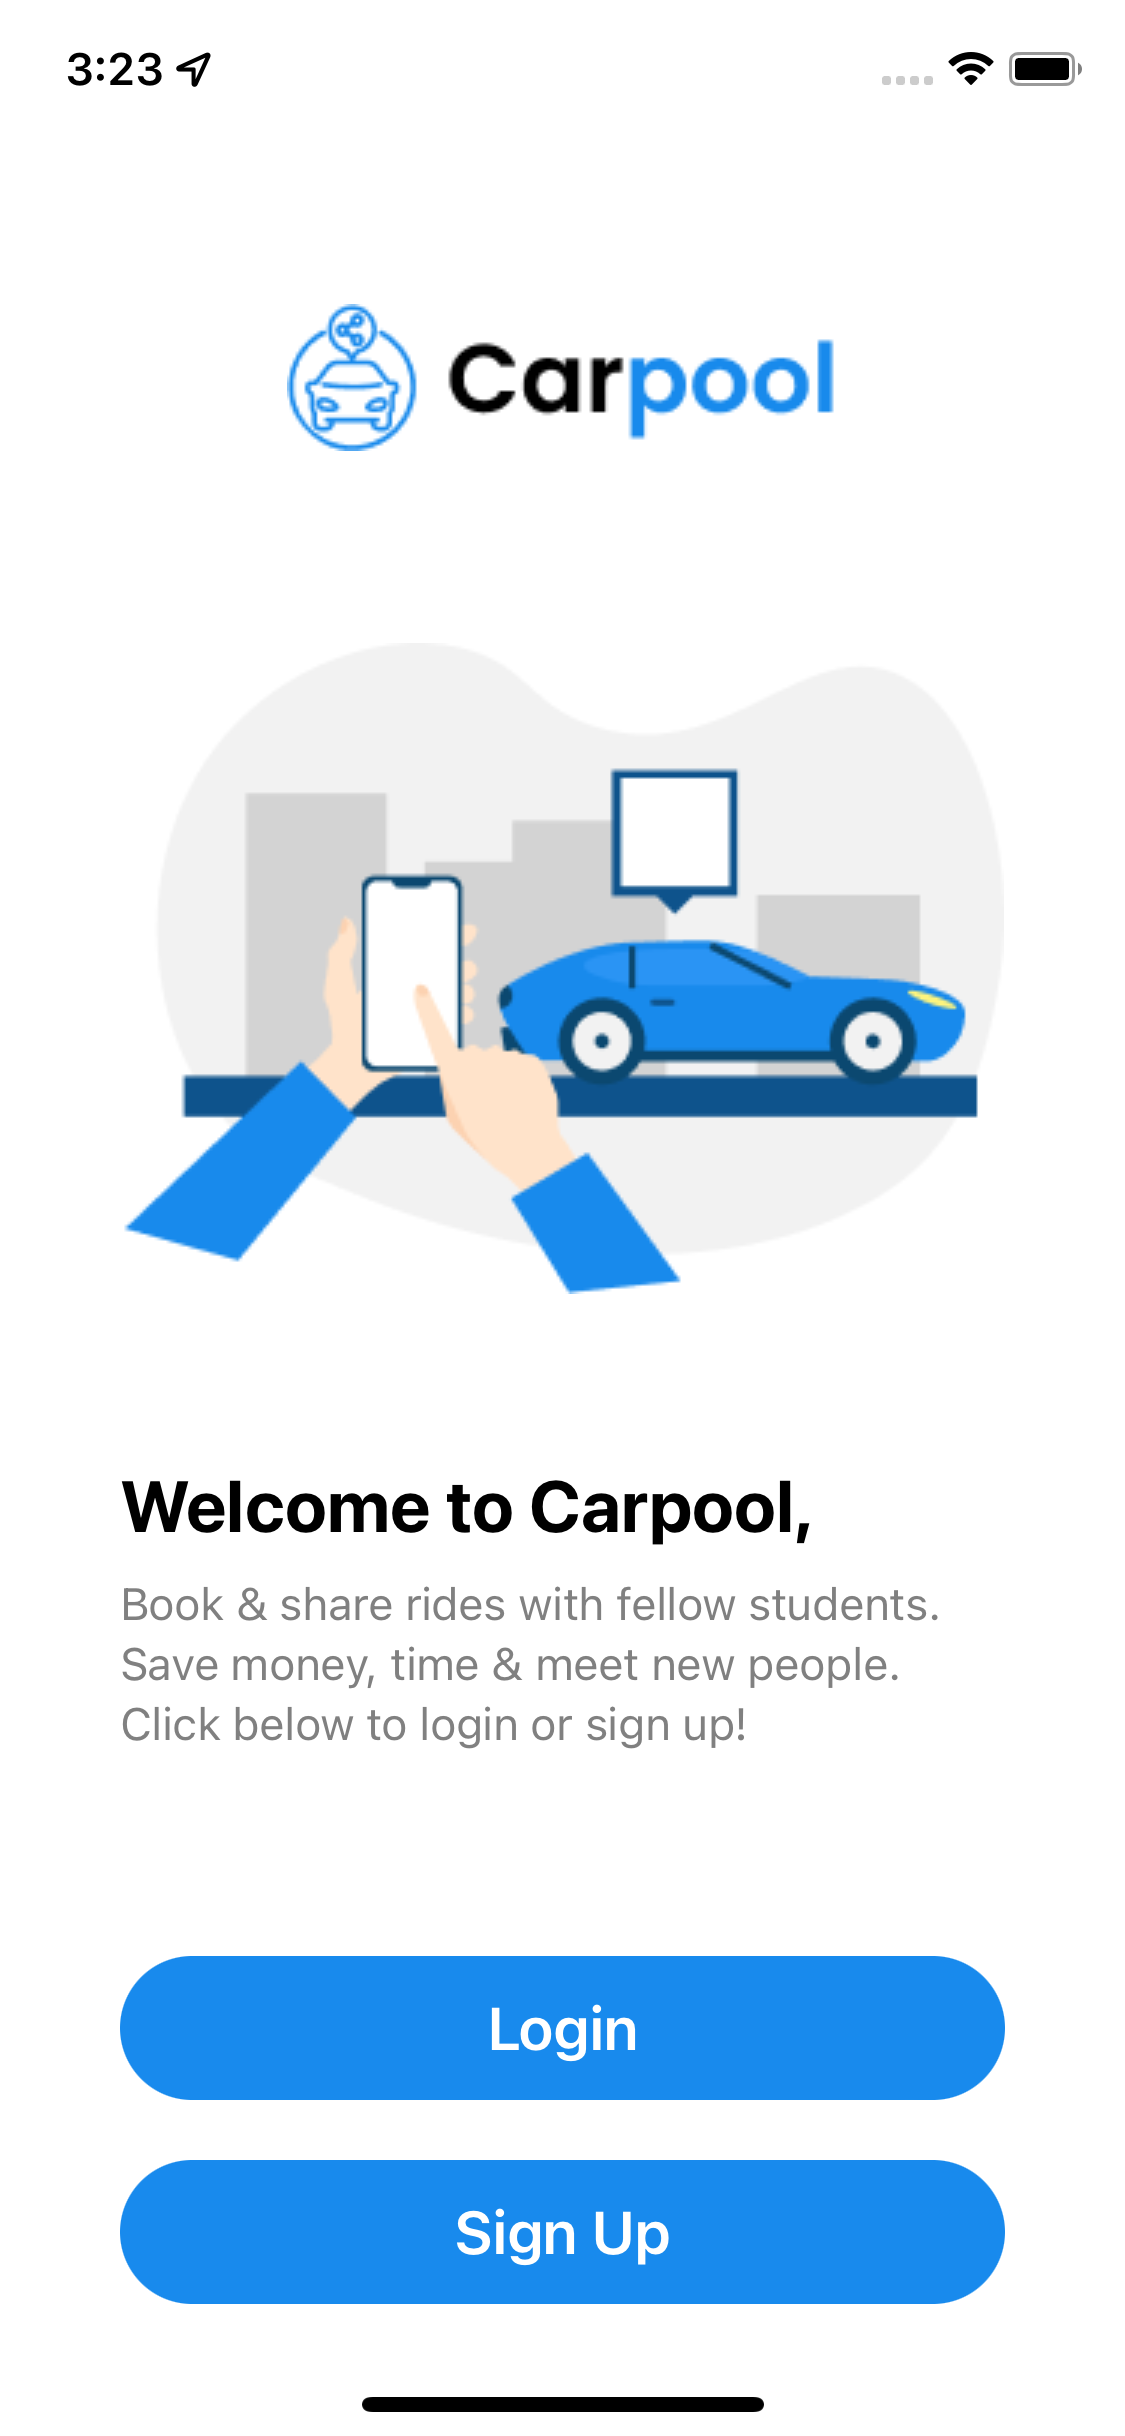
\includegraphics[height=10cm]{images/Simulator Screen Shot - iPhone X - 2022-06-10 at 03.23.06.png}
\end{center}
\subsubsection{Login Page}
When you click the login button on the landing page, you will be directed to this login page. You will be required to enter your email address and password (keyboard input) in the input text boxes labelled email address and password - located in the middle of the screen. Once you have completed the necessary information, you may click the blue Login button located at the bottom of the page.
\begin{center}
  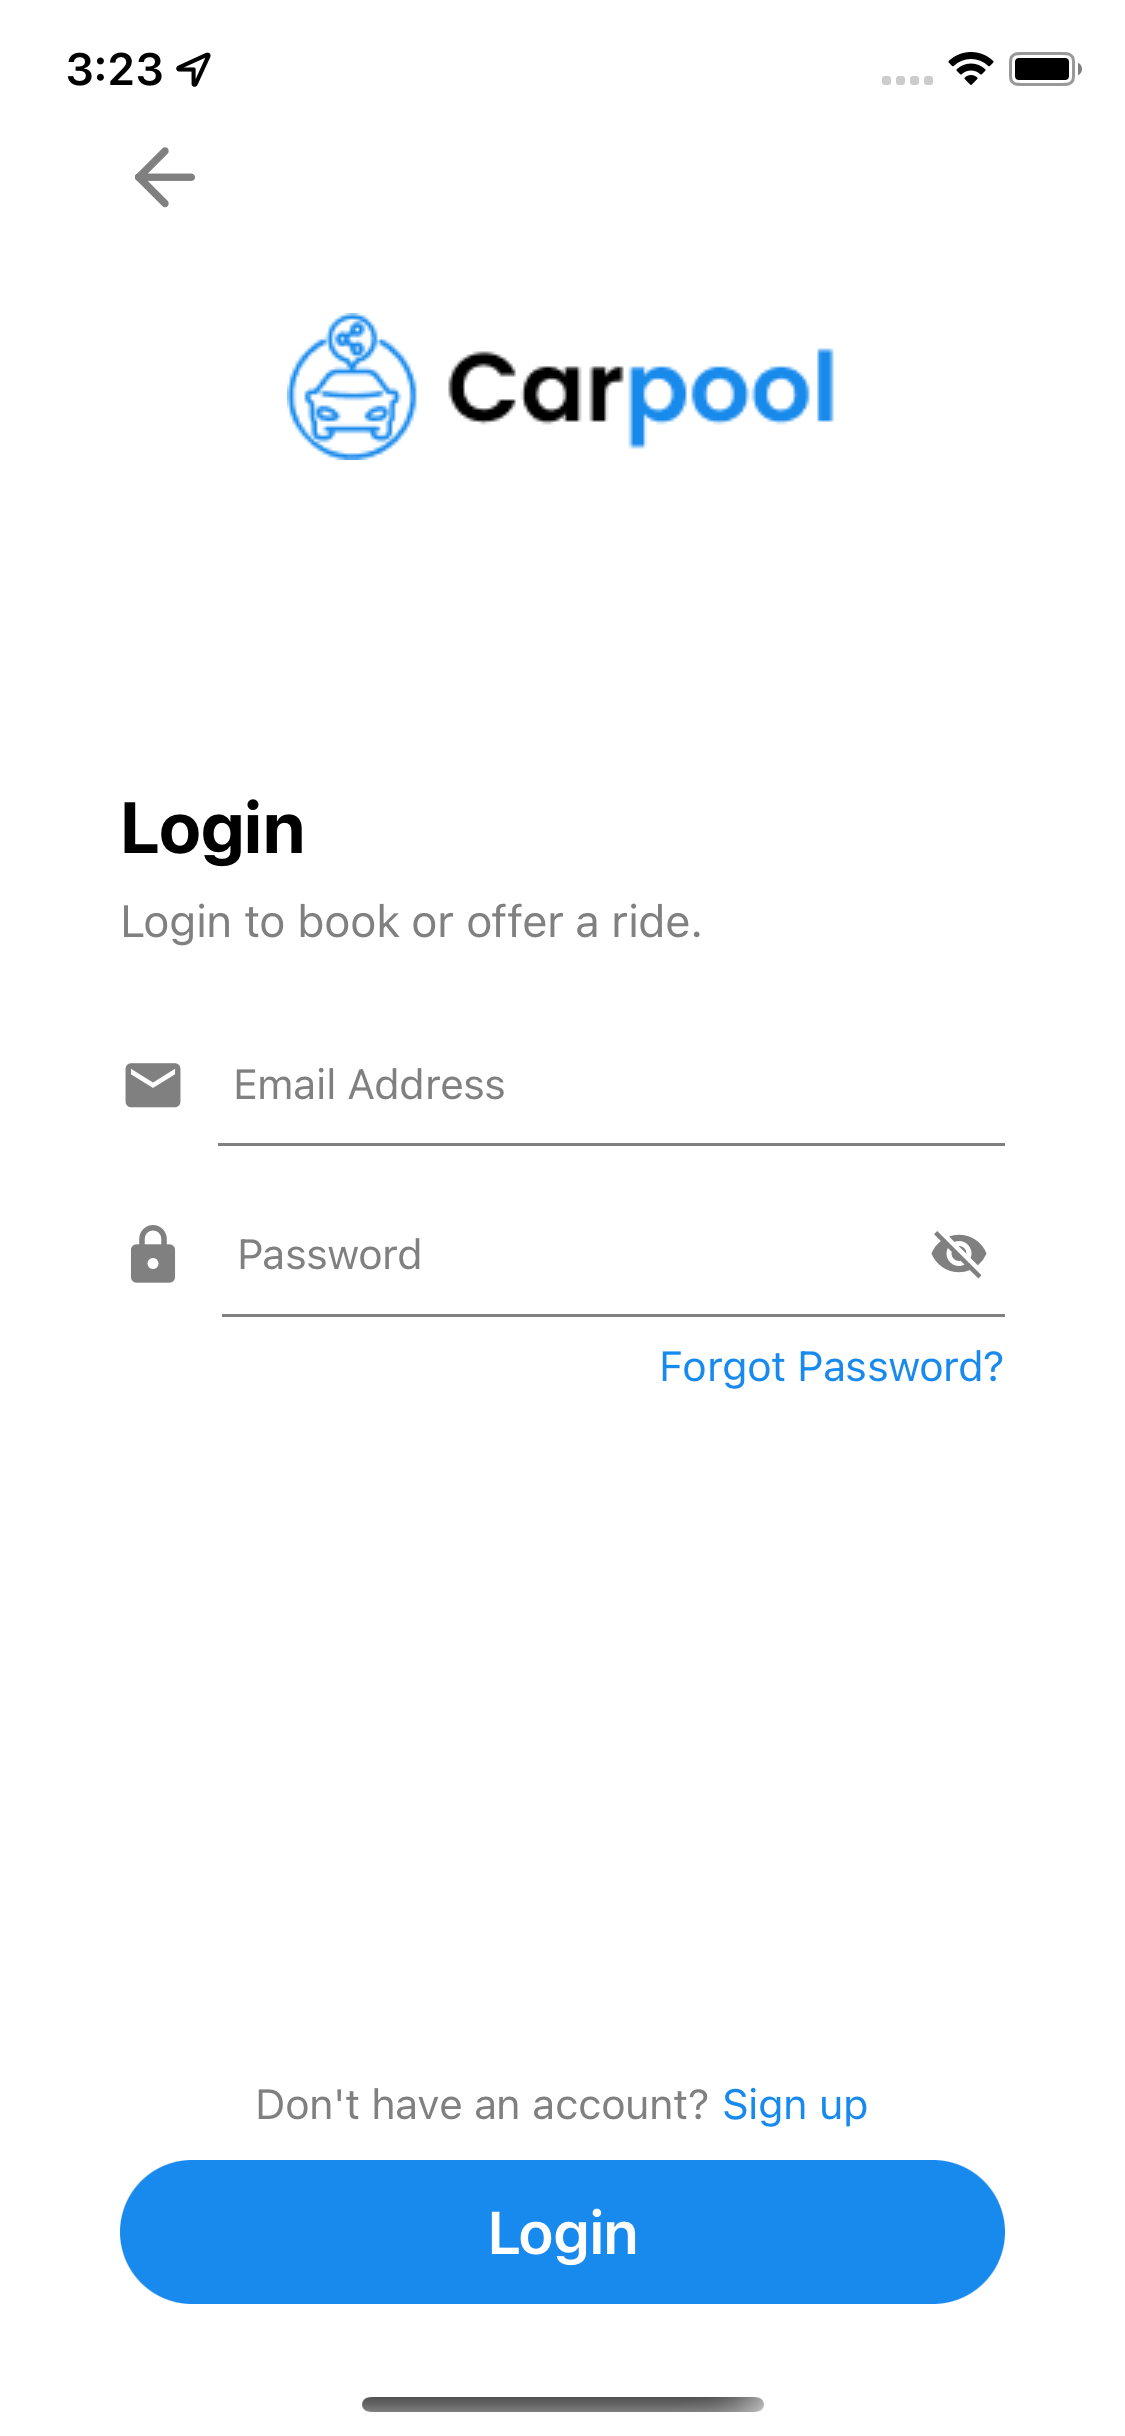
\includegraphics[height=10cm]{images/Simulator Screen Shot - iPhone X - 2022-06-10 at 03.23.09.png}
\end{center}
\vspace{1cm}
\subsubsection{Sign-up}
If you clicked the SignUp button on the landing screen, you will be directed to this page. You are asked to enter personal information via the input boxes that are displayed on the screen. Once you have entered your information, and verified that it is correct, you can click the blue signup button which is located at the bottom of the screen.
\begin{center}
  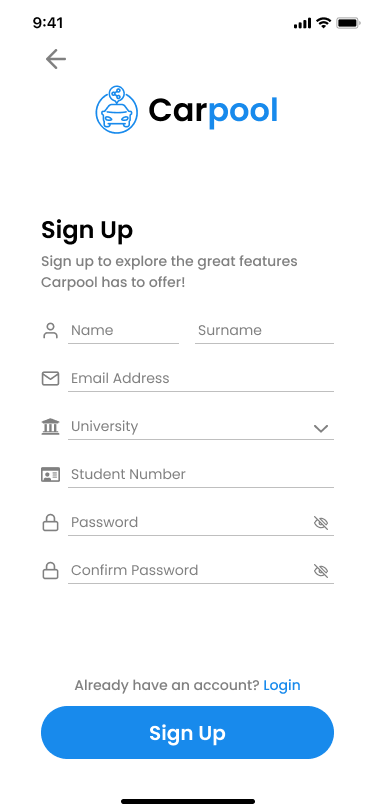
\includegraphics[height=10cm]{images/Register.png}
\end{center}
\vspace{1cm}
\subsubsection{Forgot Password}
If the you forget your password, you will not be able to log into the application. On the login page you are provided a link "forgot password" under the password text box. If you click that link you will be directed to this page, where you will be asked to enter your email address that you have registered your account with. You will then be sent a link which will allow you to reset your password.
\begin{center}
  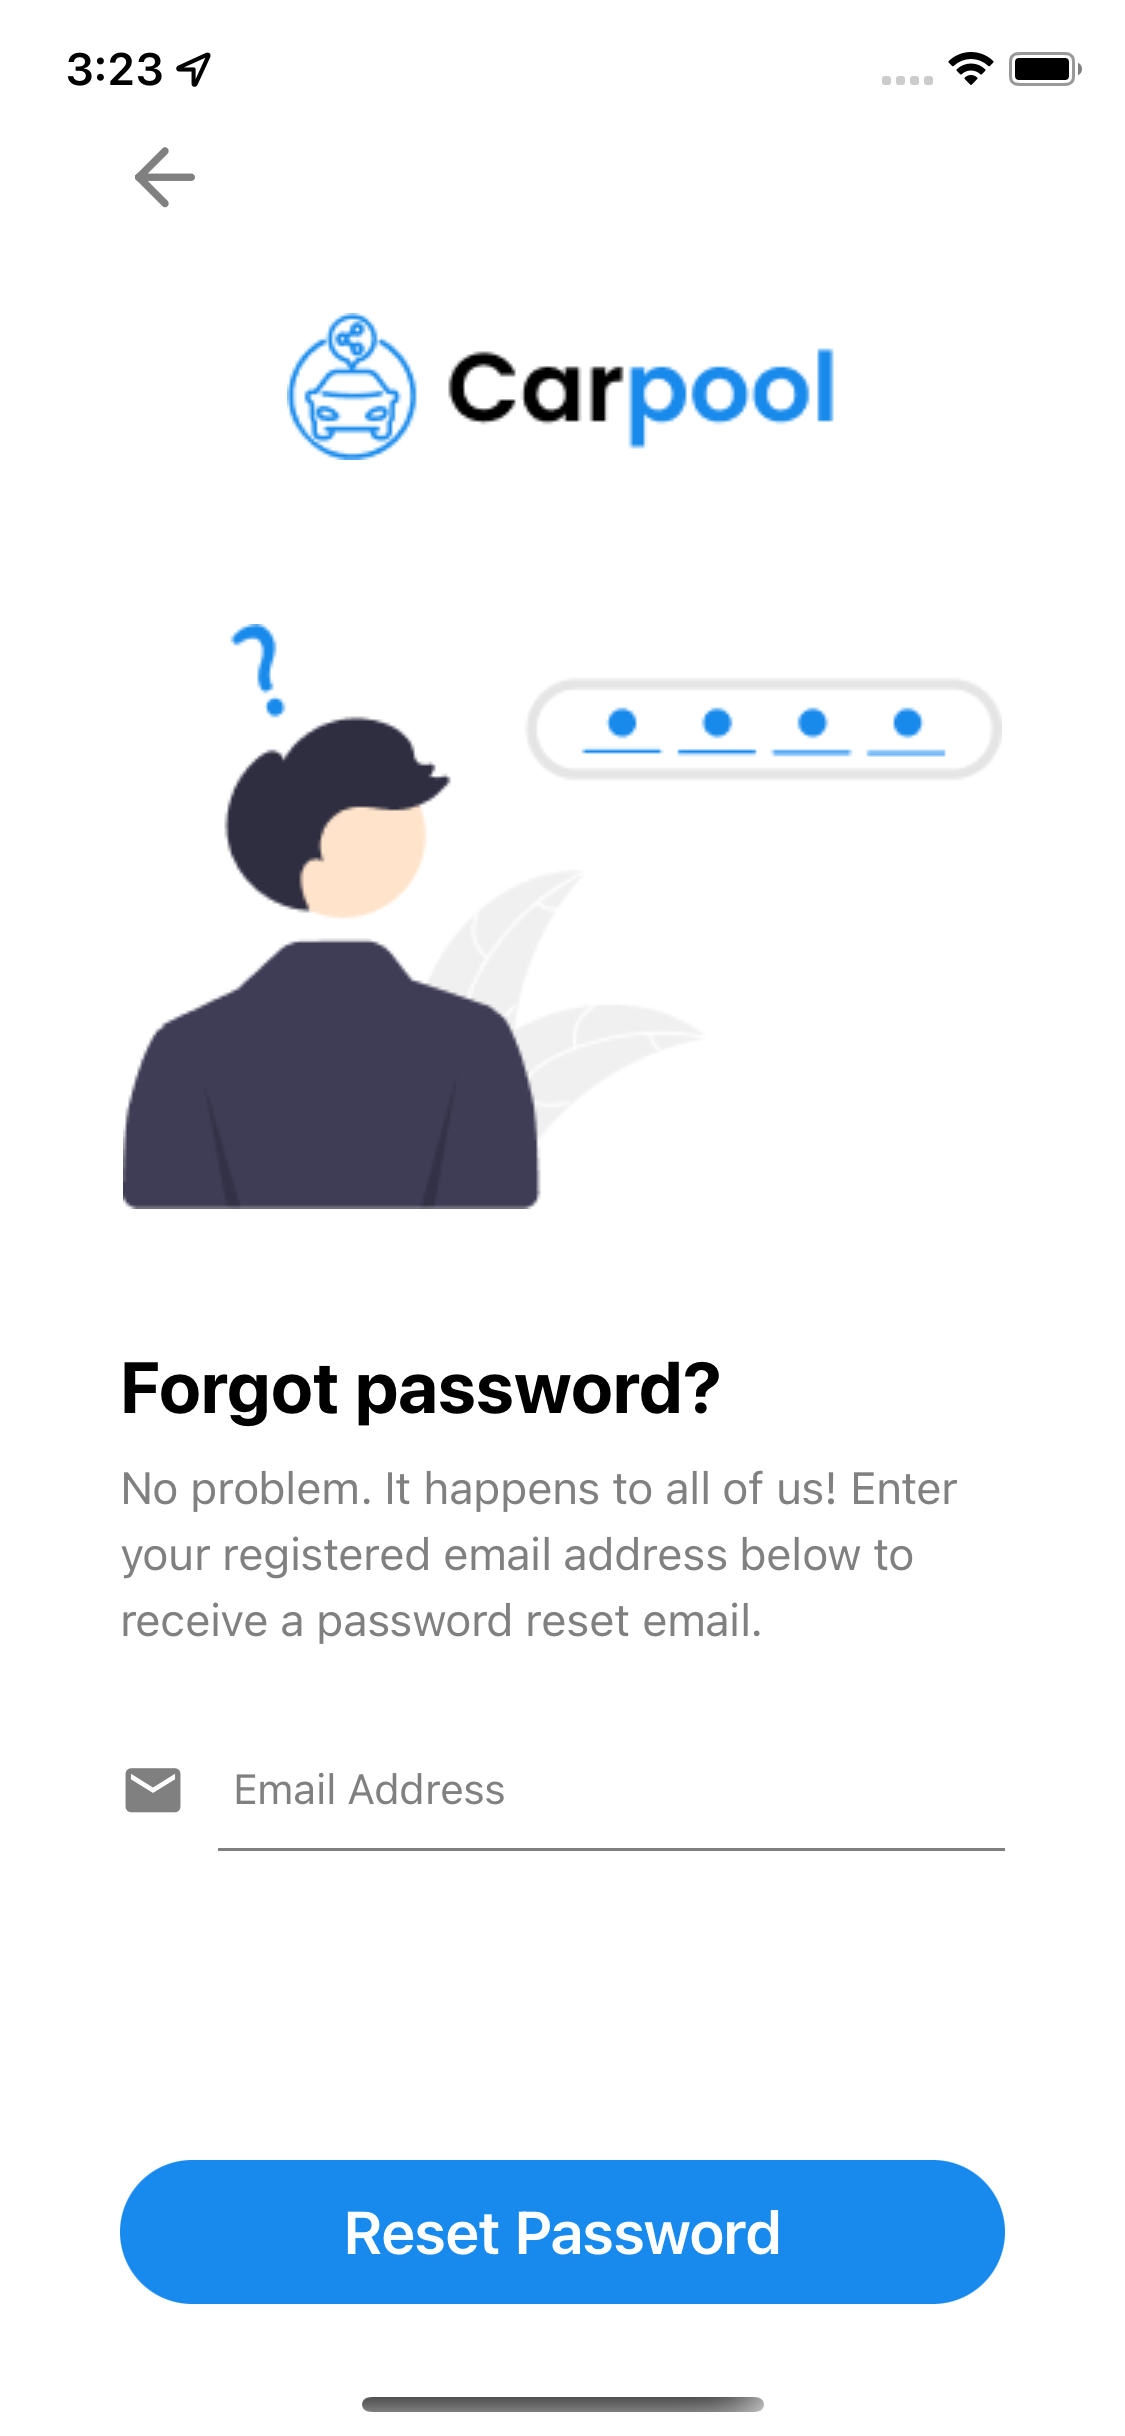
\includegraphics[height=10cm]{images/Simulator Screen Shot - iPhone X - 2022-06-10 at 03.23.17.png}
\end{center}
\vspace{1cm}

\subsection{Trips}
\subsubsection{Trip Homepage}
When you have logged in successfully you will be directed to the homepage of the carpool application.
On the homepage, the user is able to:
\begin{itemize}
  \item Search for trips by clicking on the search bar which is located at the top of the page ( oval bar that has a magnifying glass)
  \item Find a Trip   by clicking the white button in the middle of the screen titled “Find a trip”
  \item Create a Trip   by clicking the white button (below the Find a Trip button) which is located in the middle of the screen titled: “Create a Trip”
  \item Make a payment for one of their existing trips, by clicking on the shopping cart which is located next to the search bar.
\end{itemize}\\
The map that is displayed on the homepage is interactive, allowing the user to view different locations on the map by clicking and dragging different points on the map. The location that is displayed on the map is based on the user’s location.\\ \\
The user’s upcoming trip   is also displayed on the homepage (below the map). \\ \\
At the bottom of the homepage there is a navigation bar with two links:\\
\begin{itemize}
    \item Home – When clicked it will direct the user to the homepage (current page)
    \item Profile – When clicked the user will be directed to their profile page, where they will be able to view their profile, previous trips, edit their profile, change their password and sign out.
\end{itemize}
\begin{center}
  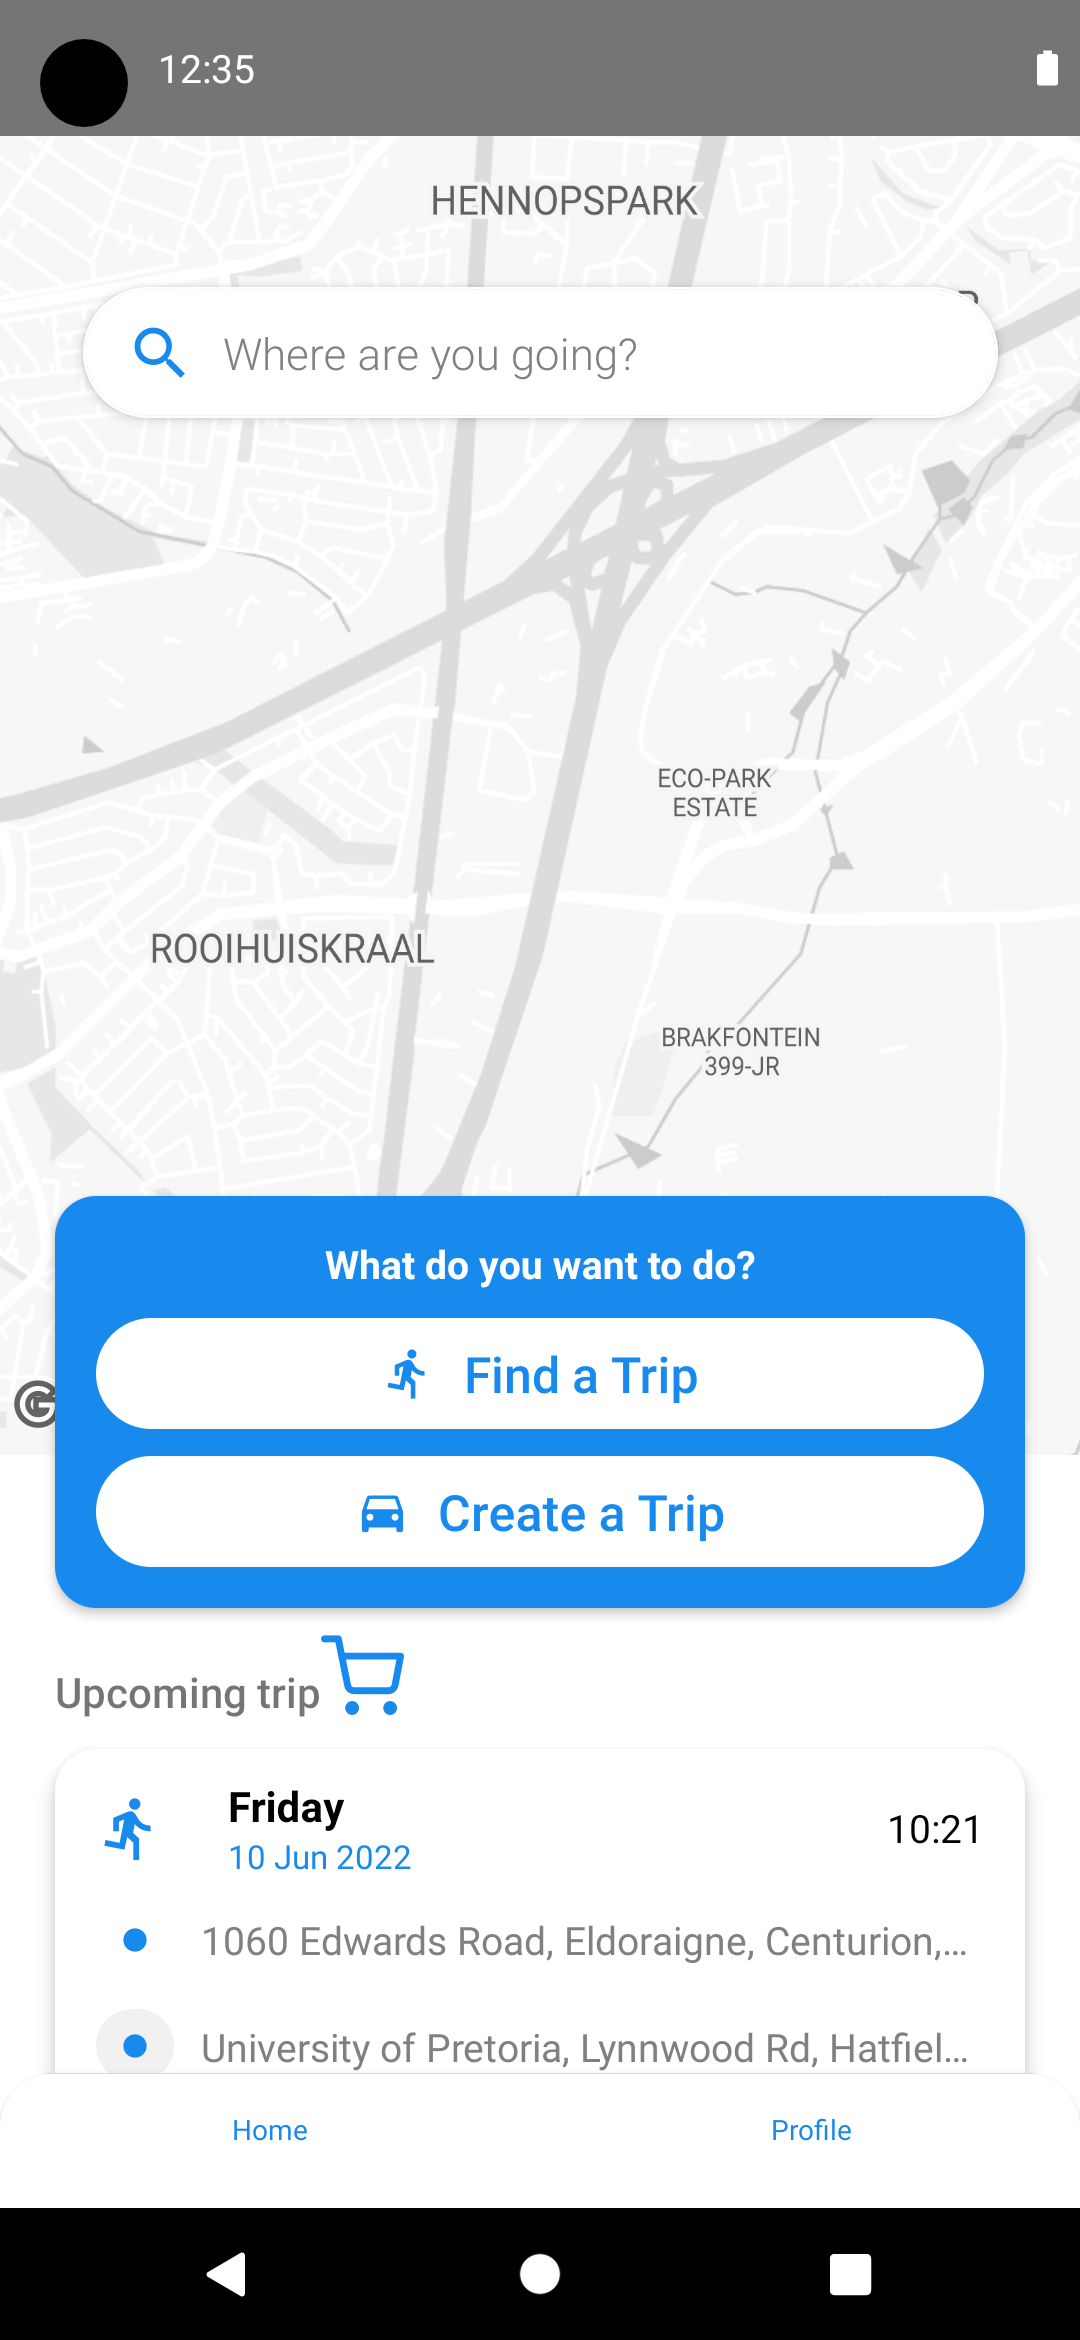
\includegraphics[height=10cm]{images/homepage.png}
\end{center}
\subsubsection{Book Trip}
On this page you are provided with the opportunity to book a trip. To book a trip all you have to do is find the trip that you are interested in and click the book button. To search for a trip that you are interested in, the user is required to enter the start and destination location as well as the date of the trip.
The book button is located below the date input box (currently being blocked by “Trip booked successfully” message)
\begin{center}
  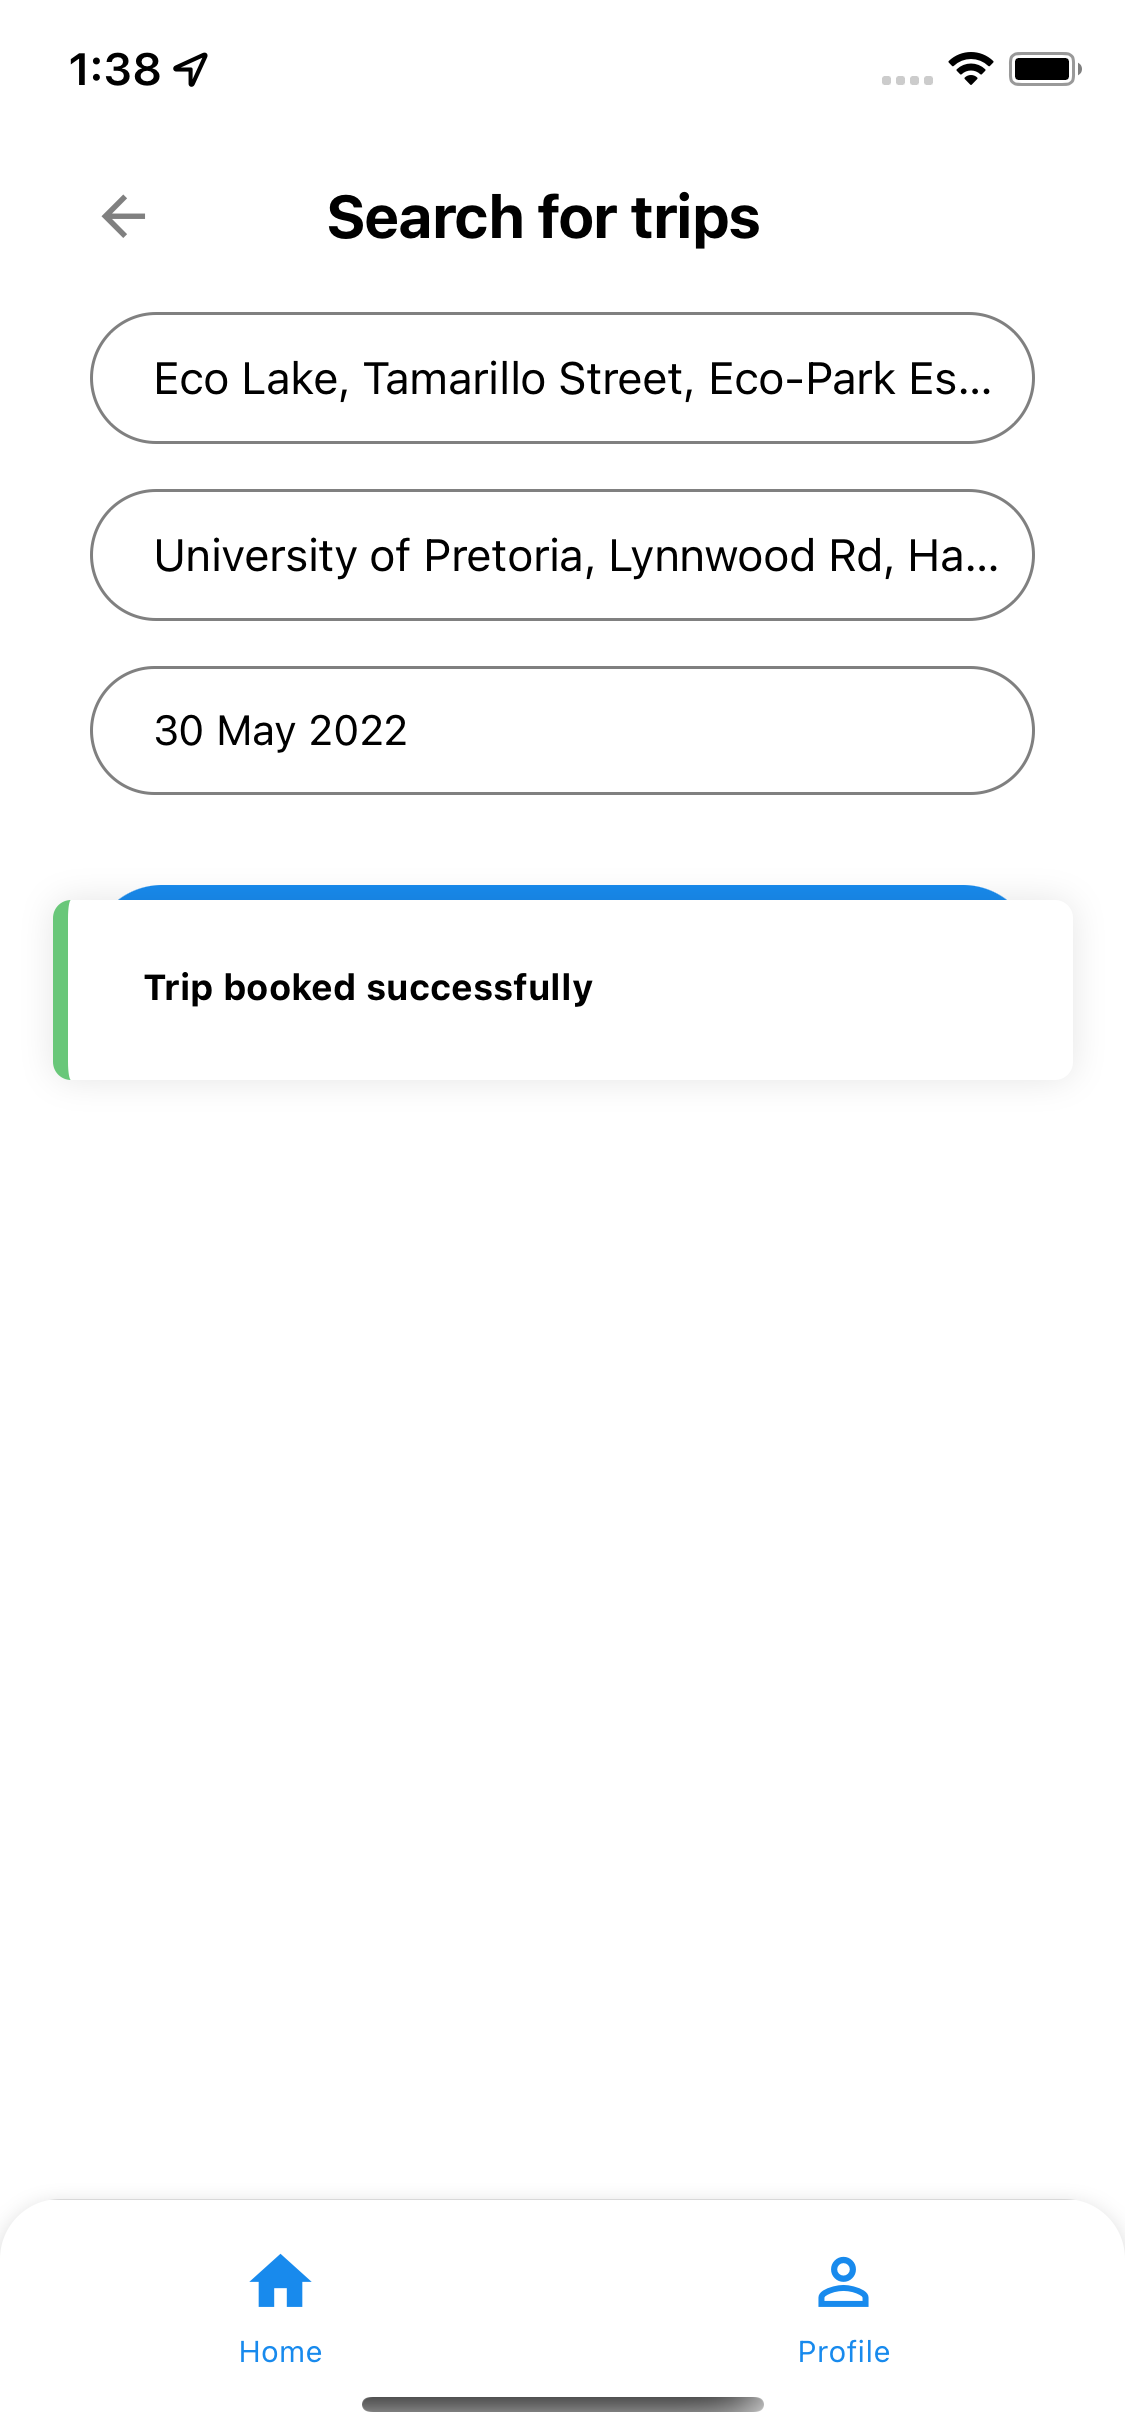
\includegraphics[height=10cm]{images/book_trip.png}
\end{center}
\subsubsection{Create Trip}
When creating a trip, the user will be asked to enter the amount of seats that are available on the trip, the cost of each seat as well as the start and end location of the trip. The user will enter this information in the respective labeled input boxes(keyboard input).By clicking the confirm button towards the bottom of the page, the user will be able to successfully create a trip. Other users of the carpool application will then be able to search and join the trip that has recently been created.
\begin{center}
  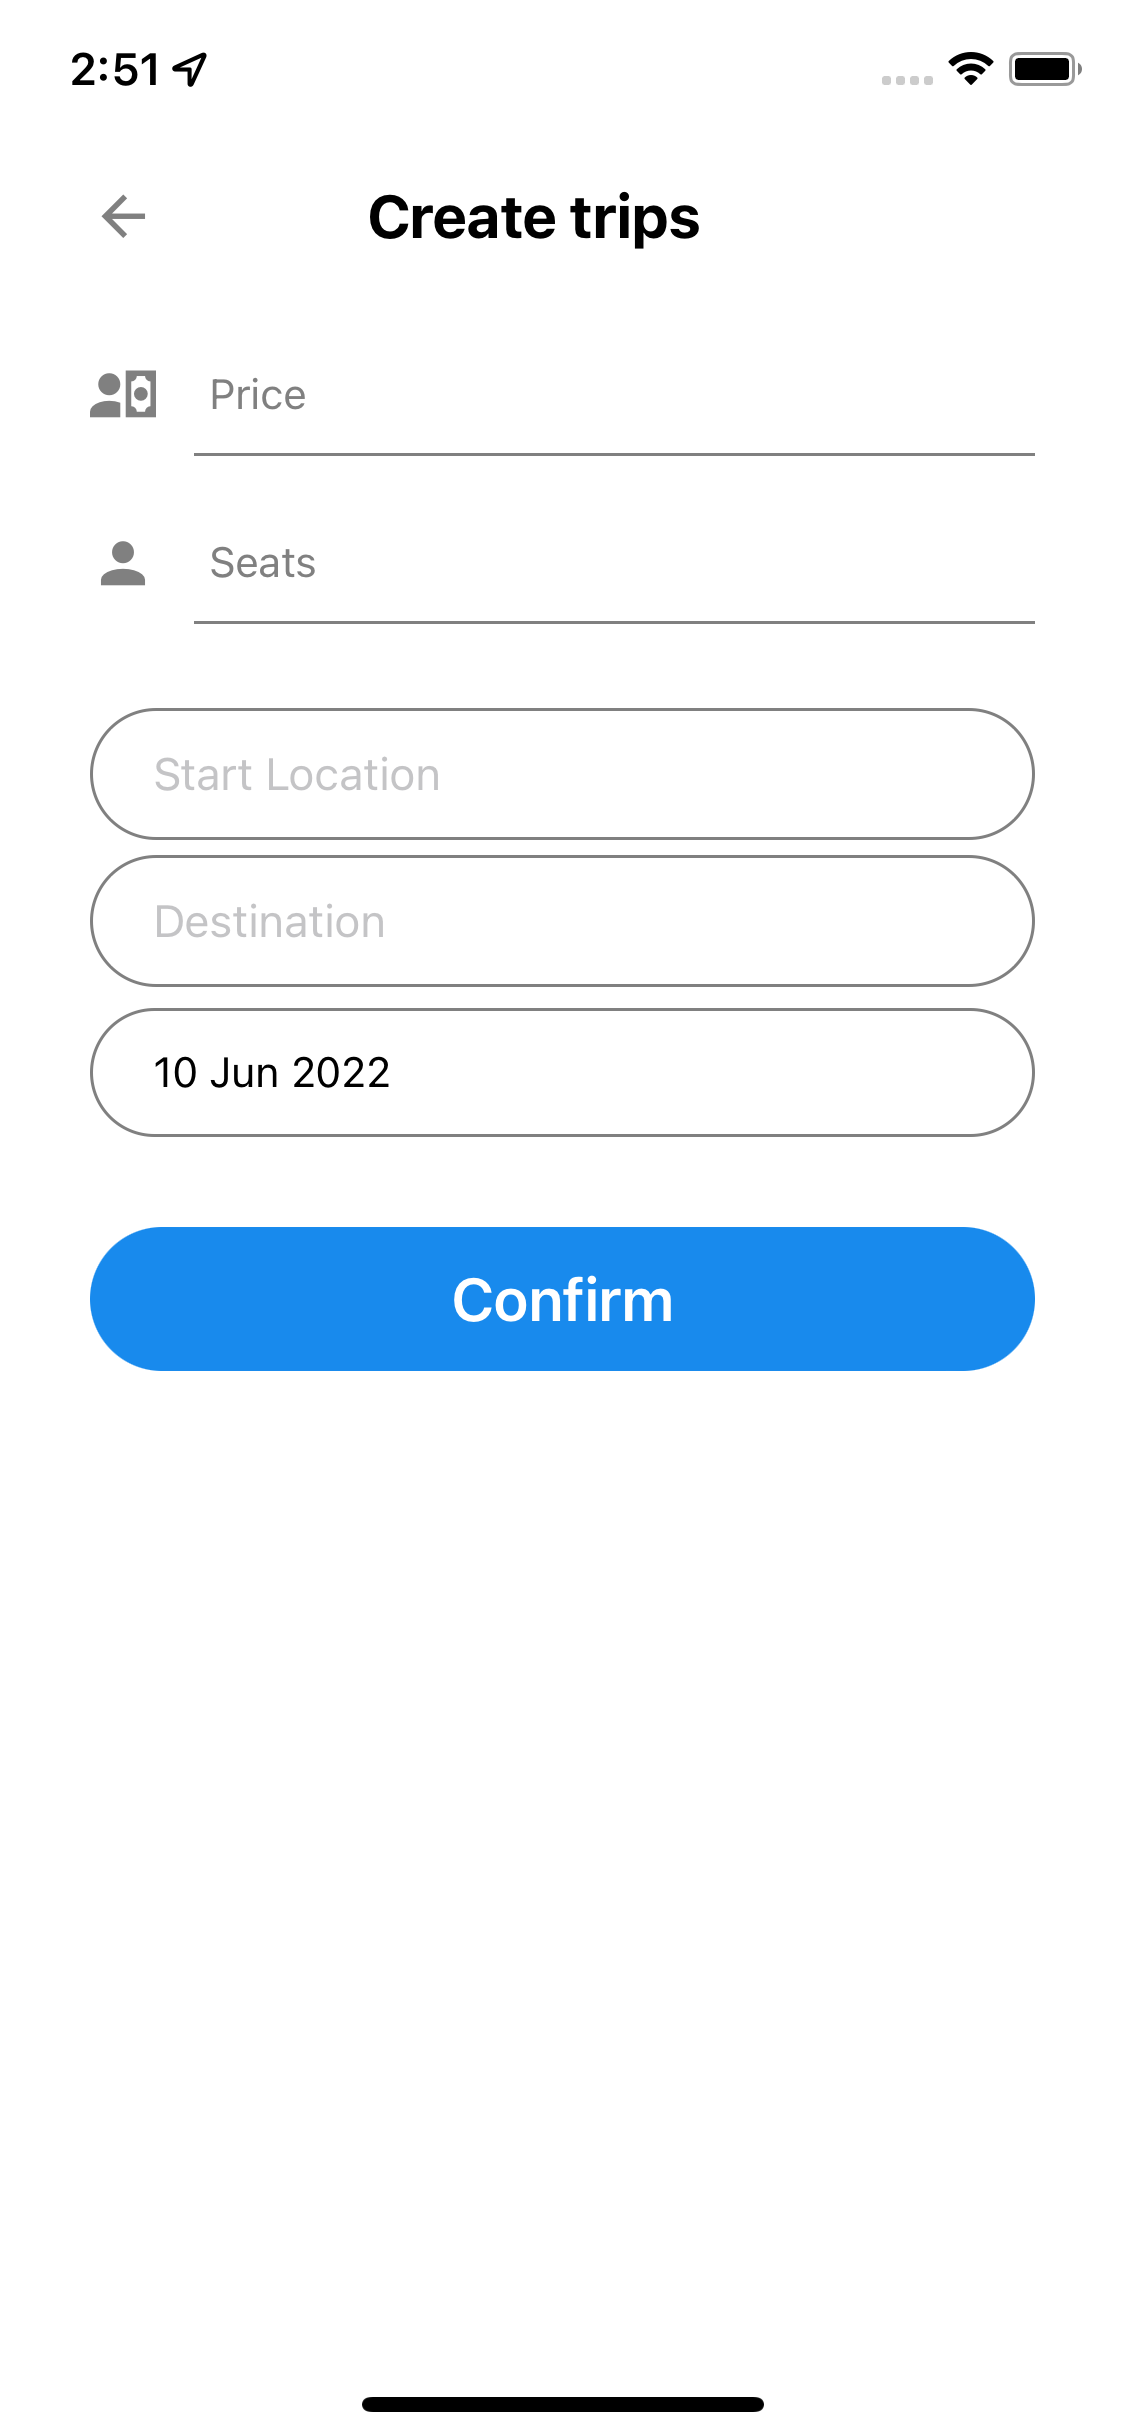
\includegraphics[height=10cm]{images/create_trip.png}
\end{center}
\vspace{1cm}
\subsubsection{Search Trip}
  In order to search for a particular trip, the user is required to enter the start and end location as well as the date of the trip. Once all this information has been entered, the user can click the search button which is located towards the upper center of the screen. When search is clicked, trips based on the information that was entered will be displayed to the user.
\begin{center}
  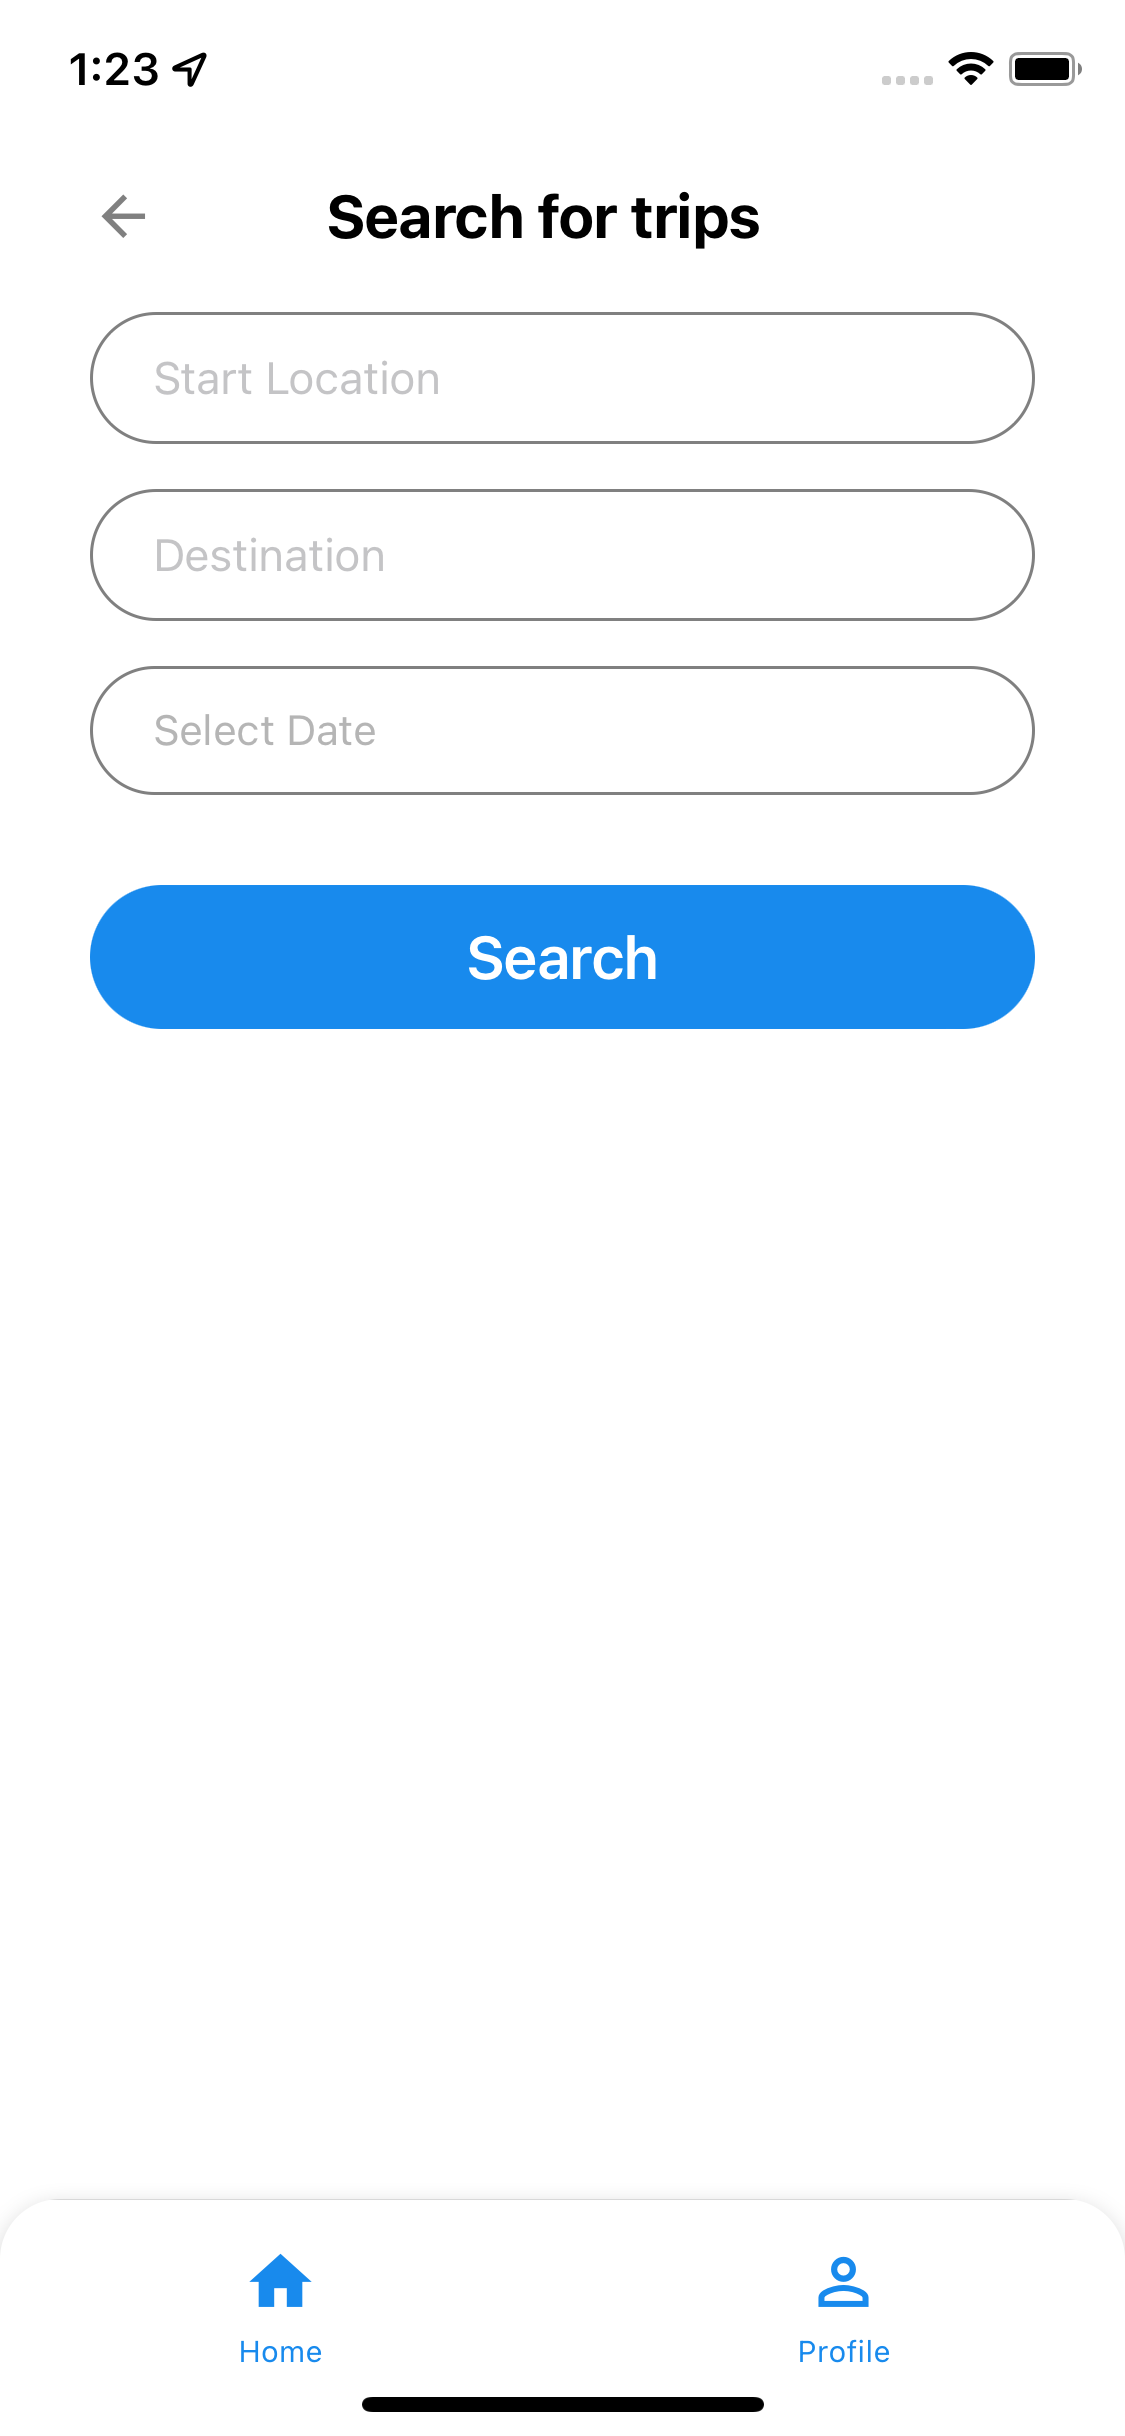
\includegraphics[height=10cm]{images/search_trips.png}
\end{center}
\vspace{1cm}

\subsection{Profiles}
\subsubsection{Profile Homepage}
The user is able to edit their information at any time. All they have to do is click on the profile icon, which can be found on the right hand side of the bottom navigation bar. The user is able to view and edit their personal information. This can be done by clicking on the profile icon, which can be found on the right hand side of the bottom navigation bar. Once the user has clicked this icon, they will be directed to the profile homepage. The user then has a choice of:
\begin{itemize}
    \item Profile – View/ Edit their personal information
    \item Trip History – View previous trips that they have created or joined
    \item Change their password
    \item Sign out
\end{itemize} \\
In order to make use of any of the above functionality, they user can click on respective buttons.
\begin{center}
  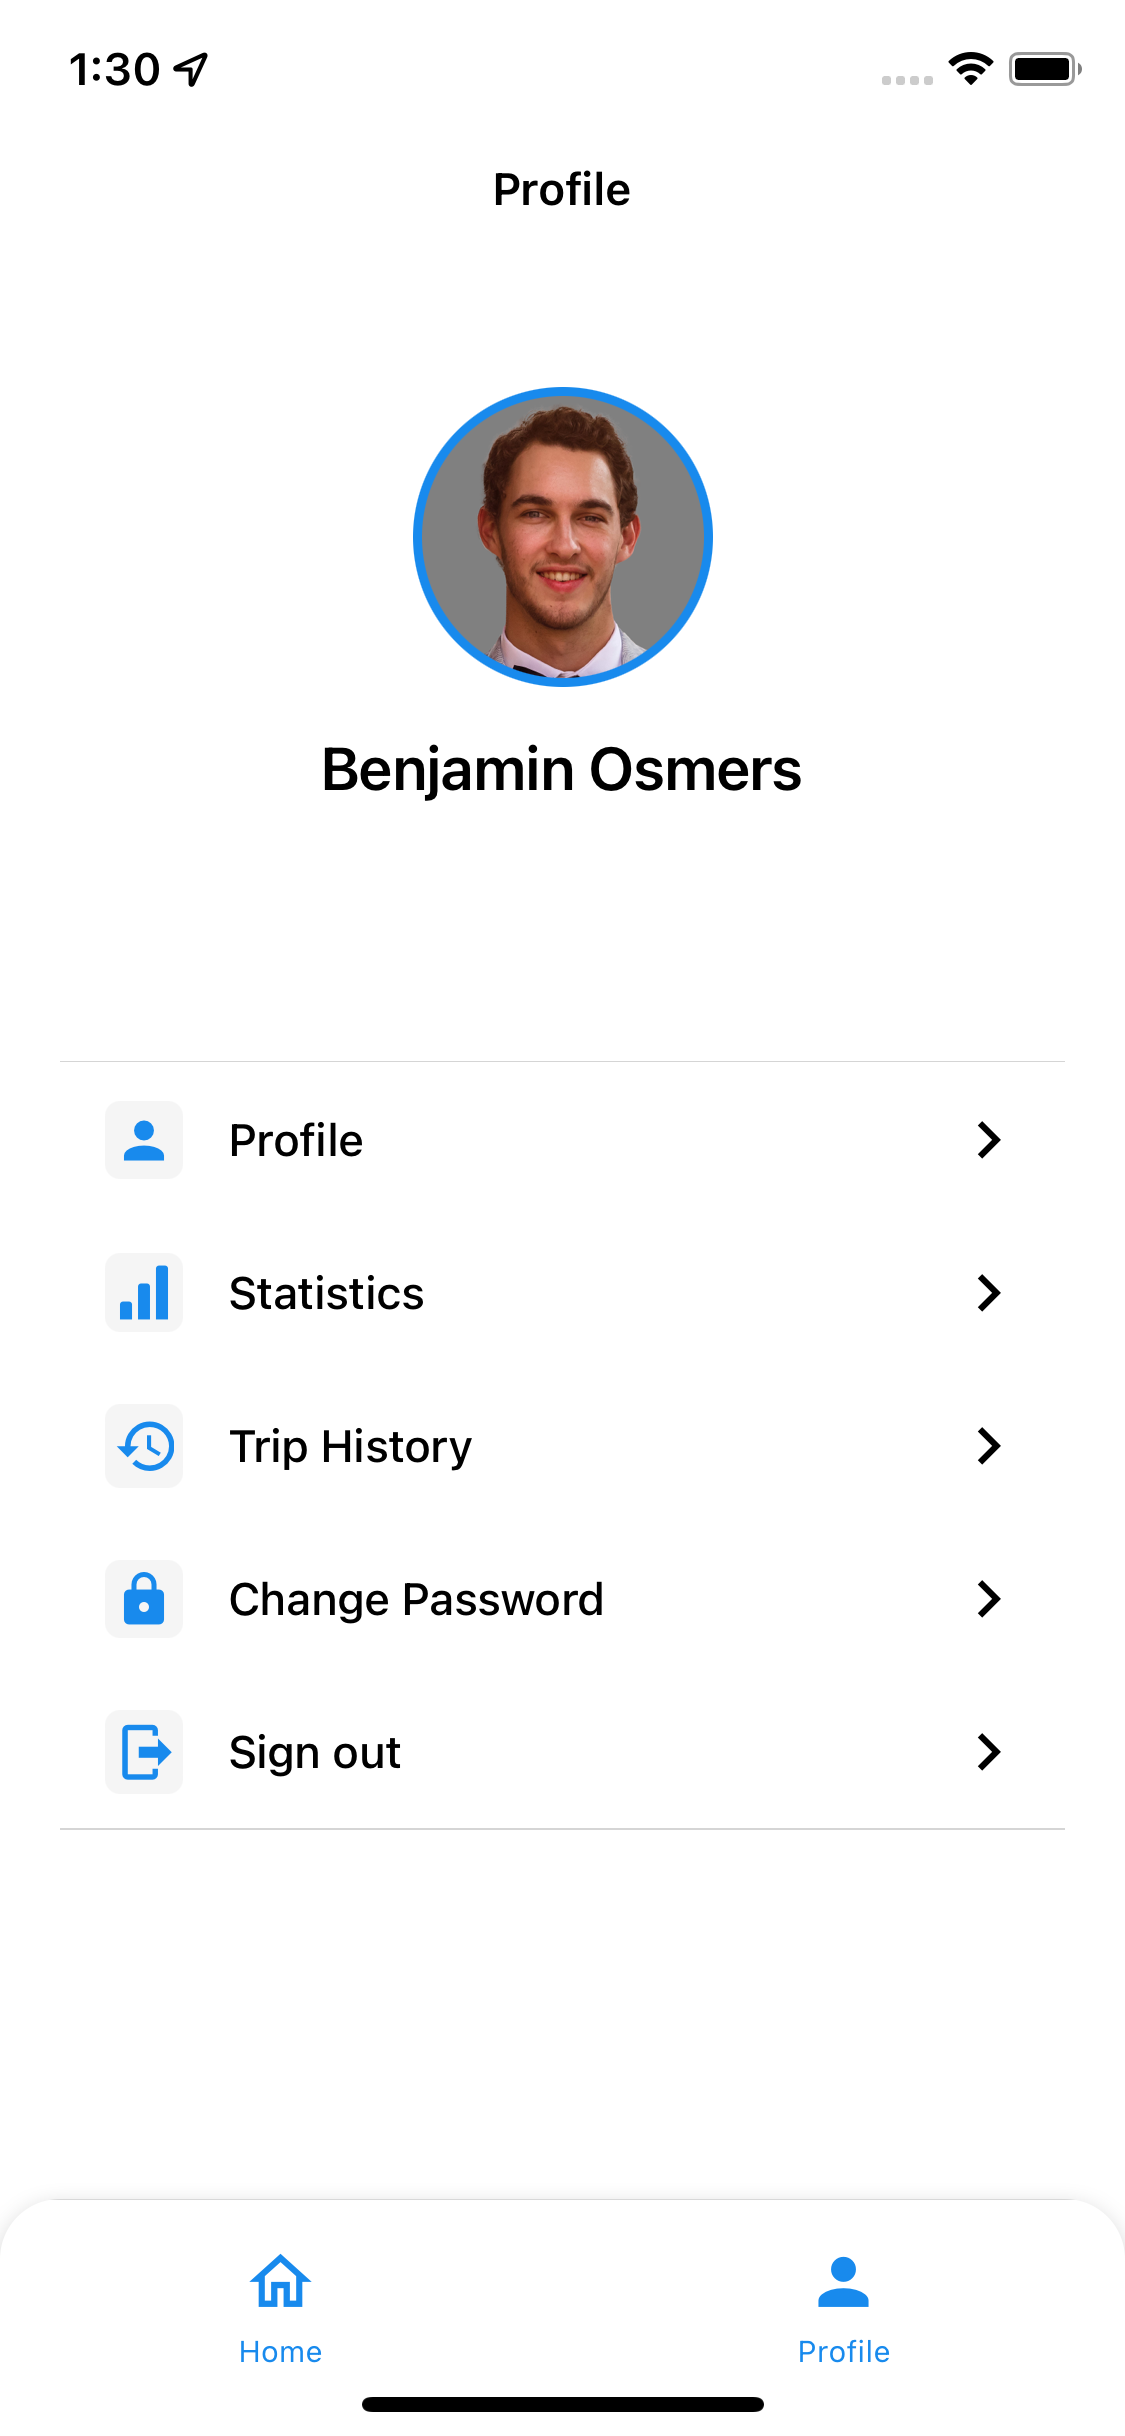
\includegraphics[height=10cm]{images/view_profile.png}
\end{center}
\vspace{1cm}

\subsubsection{Edit Profile}
The user can simply click on the information that they would like to edit, and type in the correct information (within the respective text box). Once they have corrected the information the user can click the save button which is located at the bottom of the screen. Once this button is clicked the user's information will be saved successfully.
\begin{center}
  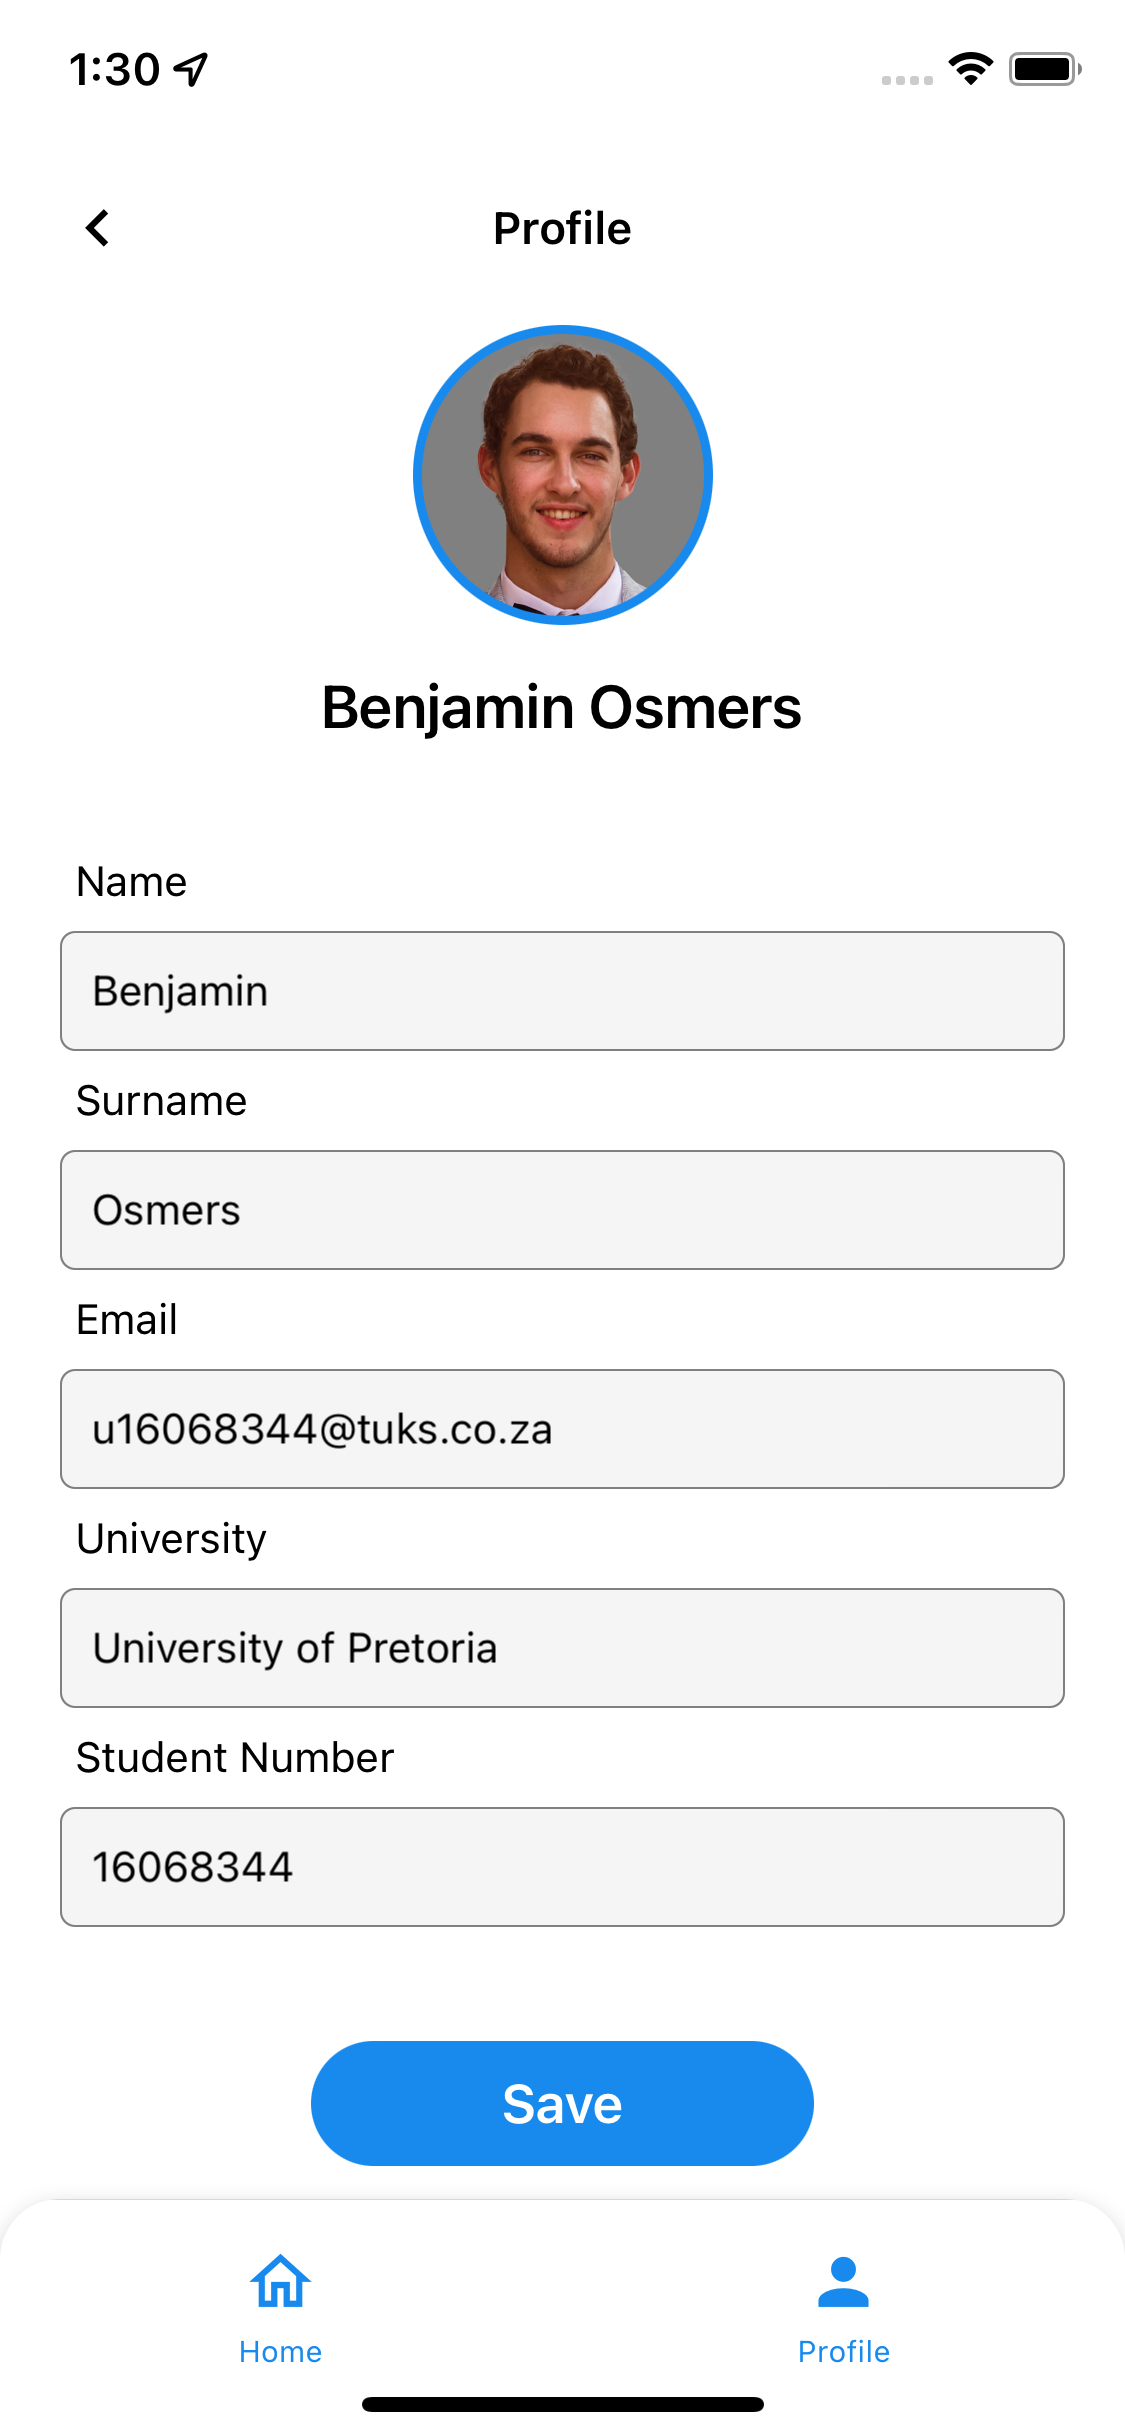
\includegraphics[height=10cm]{images/edit_profile.png}
\end{center}
\subsubsection{View Other profiles}
Users are provided with the opportunity to view other user's profiles.The user will then be able to determine if the person that they want to travel with is a good fit, and if that particular person has any bad reviews. In order to view a drivers profile, the user can just click on the drivers picture on the trip screen. They will then be directed to the driver’s profile page which displays:
\begin{itemize}
    \item The driver’s name and surname
    \item The driver’s car make and model
    \item The driver’s contact details
    \item The driver’s rating and reviews
    \item 	Provides the user with the opportunity to send a message to the driver, or to call the driver.
\end{itemize}
\begin{center}
  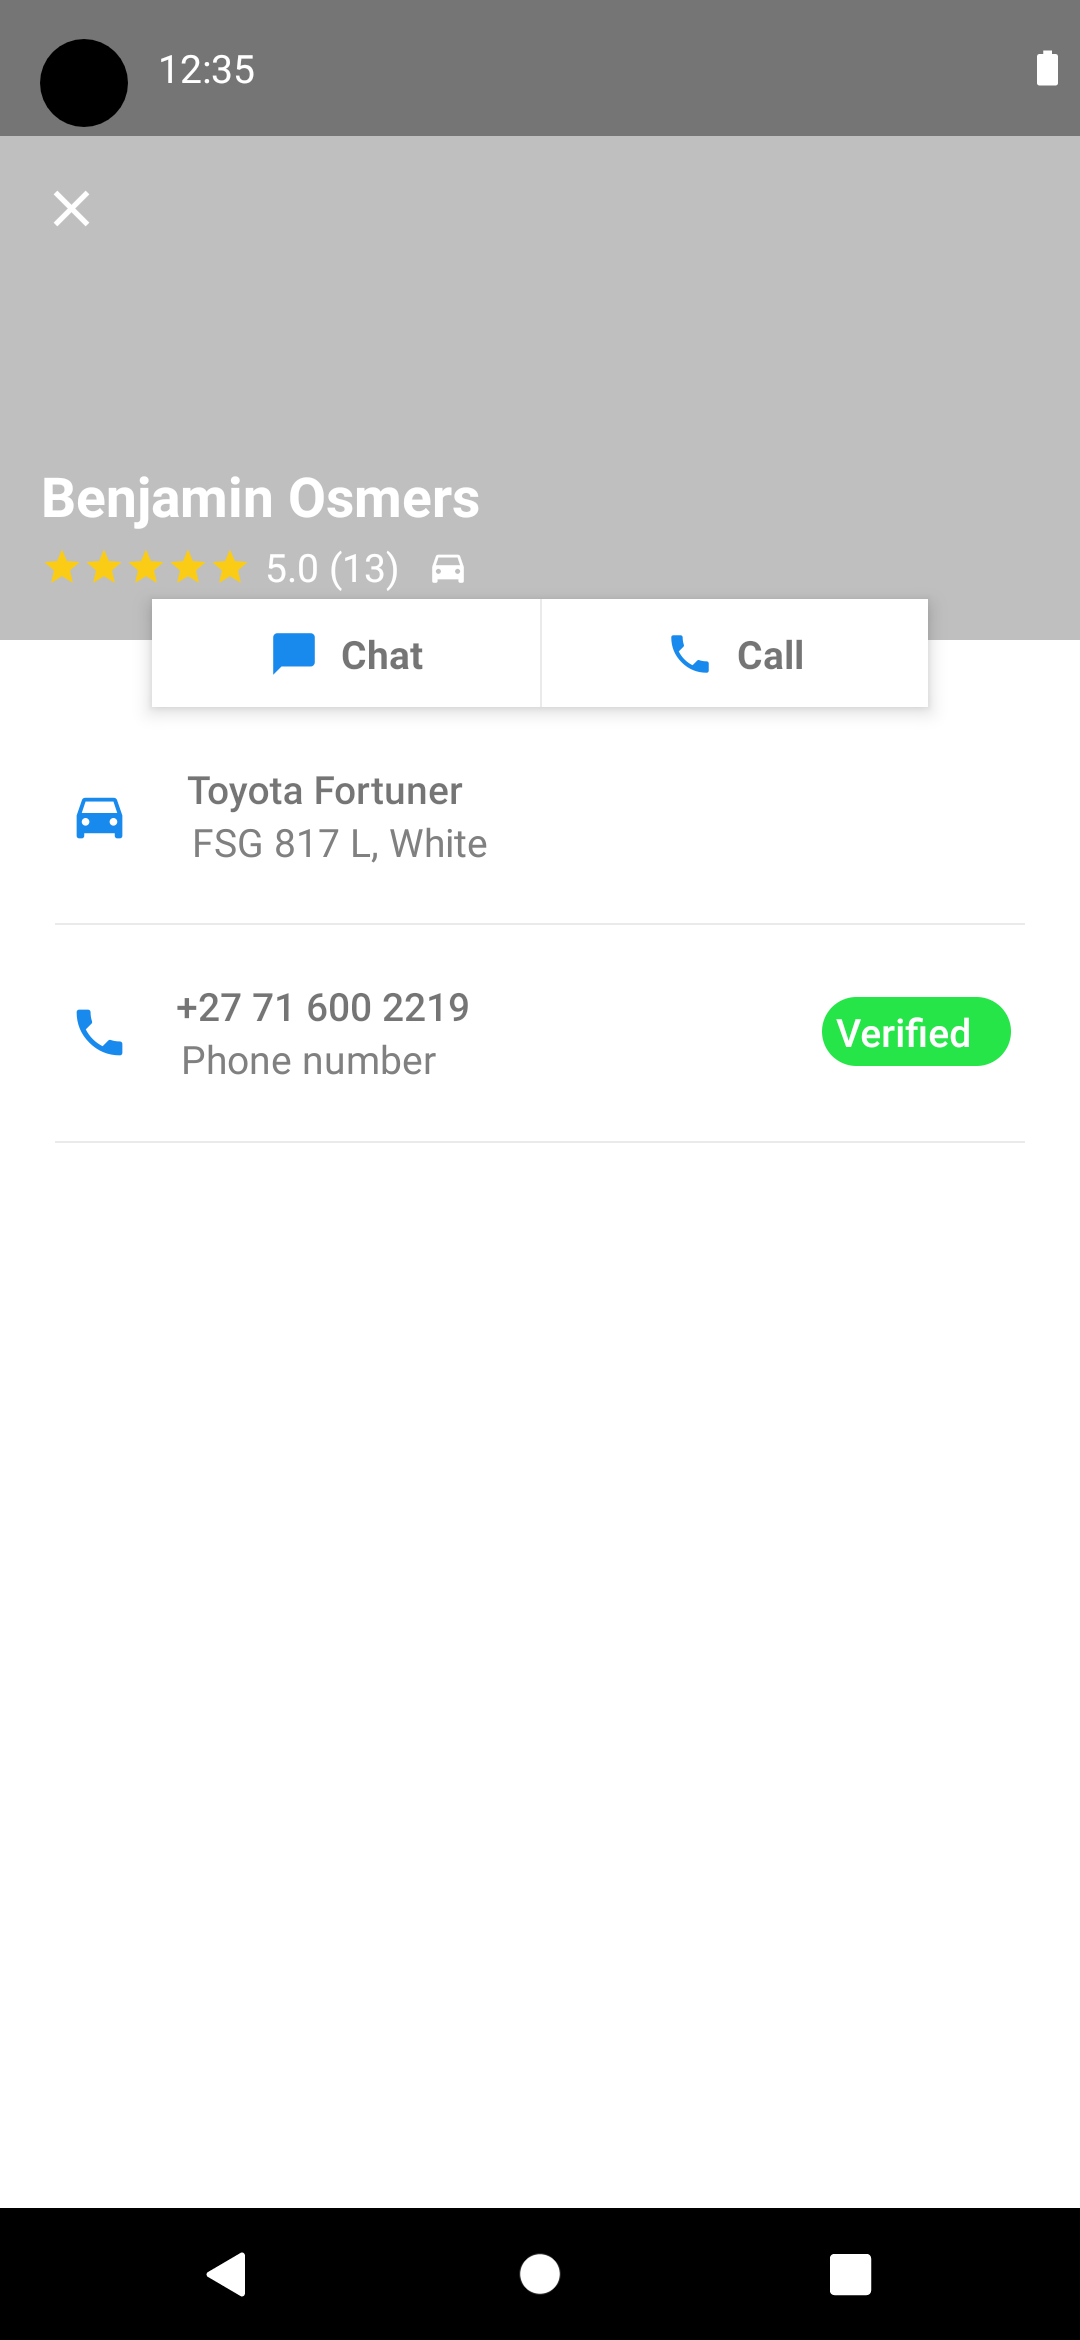
\includegraphics[height=10cm]{images/viewDriver.png}
\end{center}
\vspace{1cm}

\subsection{Trip History}
If the user clicks on the “Trip History” button which is located on the profile homepage, the user will be directed to a page that shows all the previous trips that the user has been a part of. Trip history is divided into two categories: Driver and Passenger. 
\subsubsection{Passenger History}
Passengers are able to view the previous trips that they have partaken in by clicking on the passenger tab which is located on the top of the screen. A list of previously partaken trips will appear to the user.
\begin{center}
  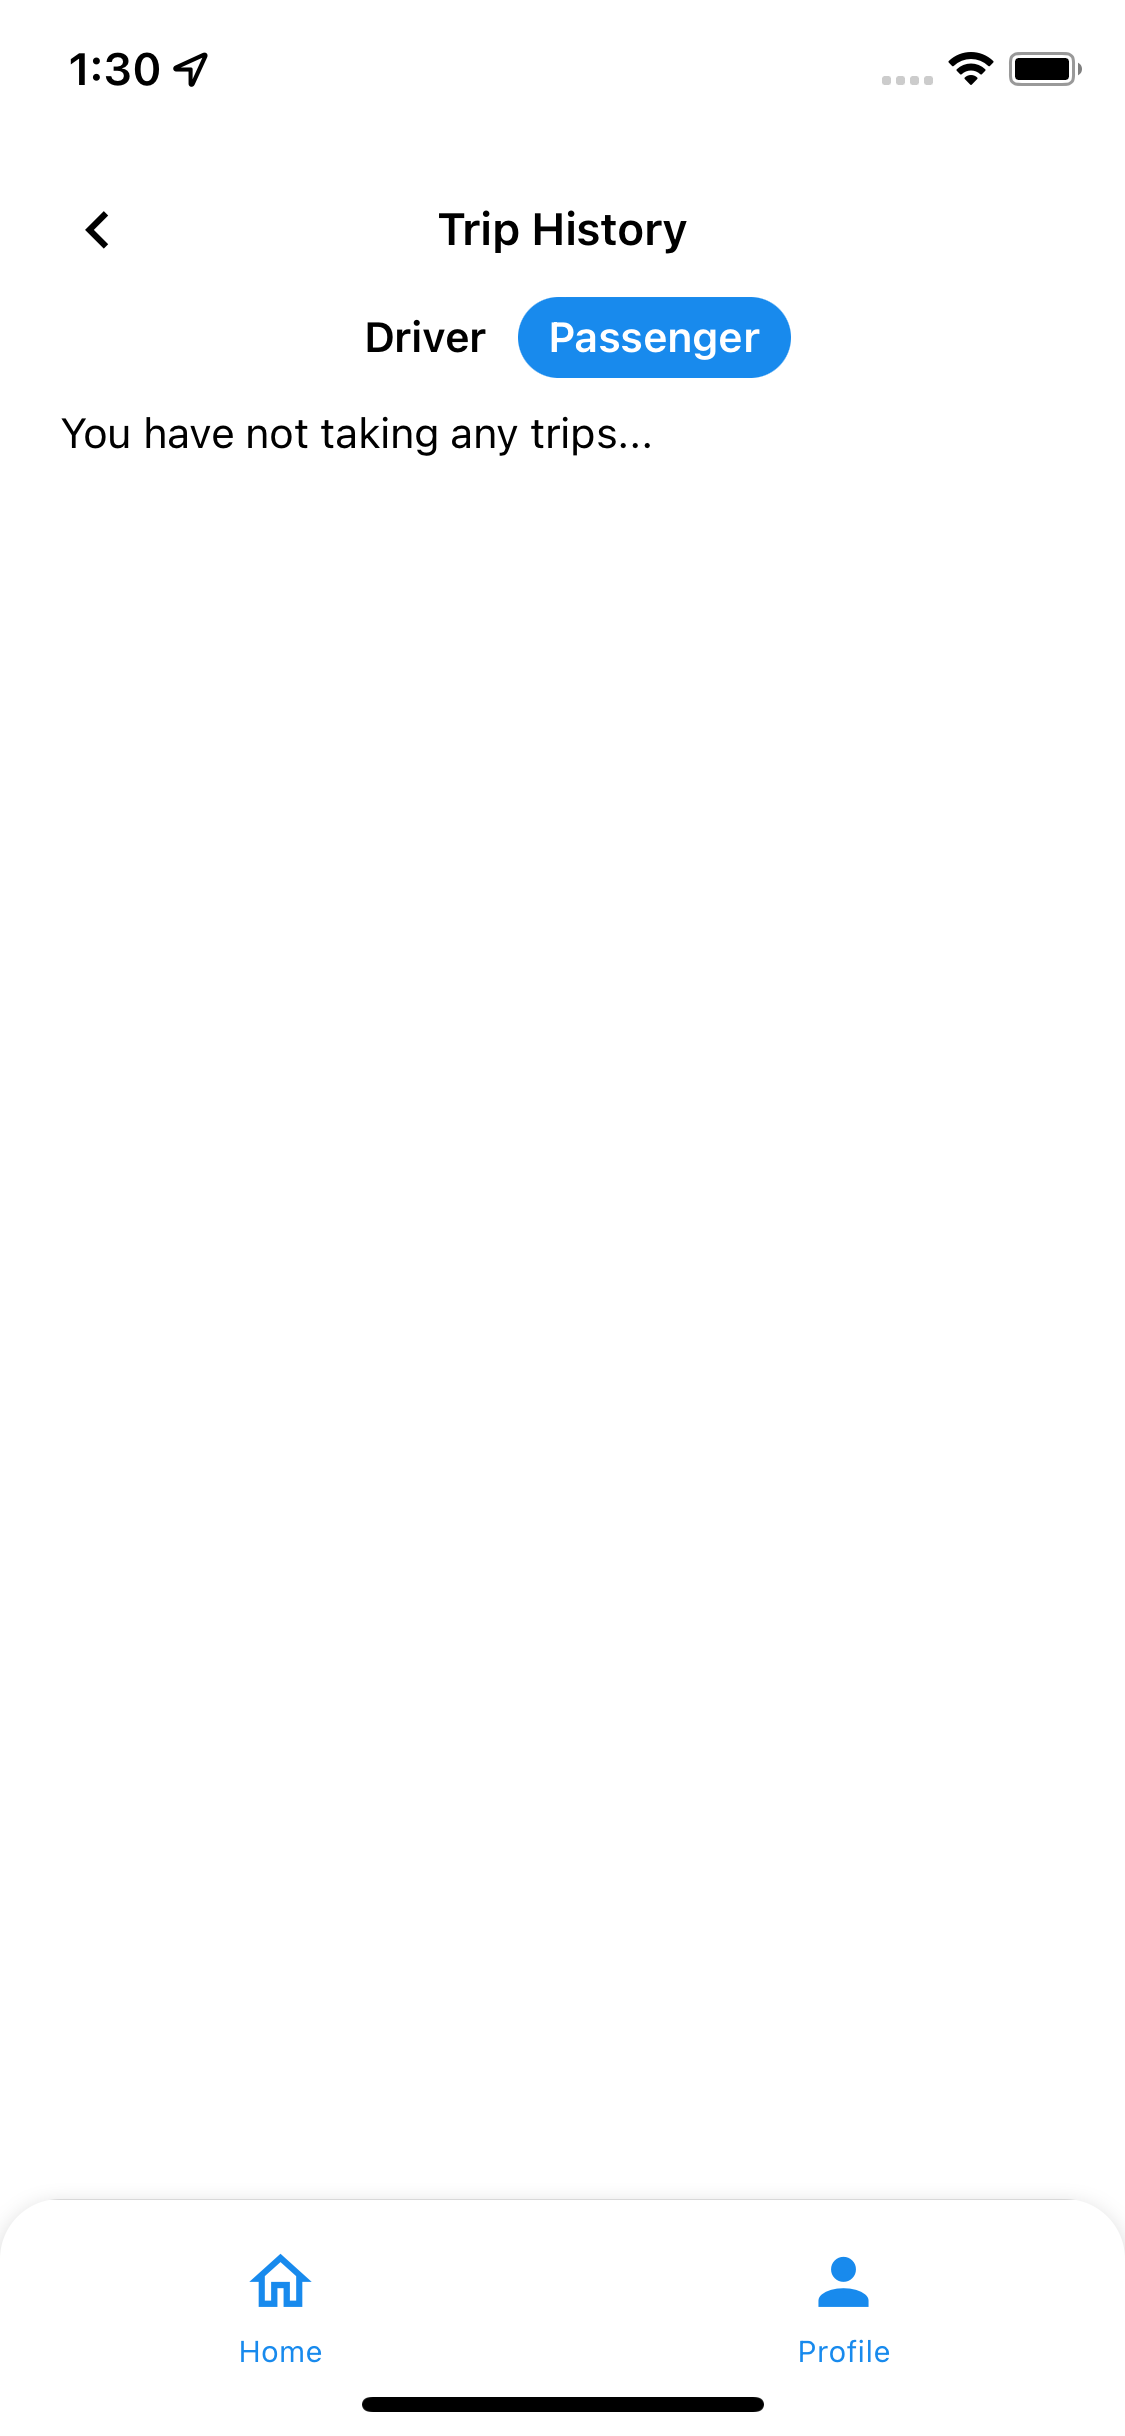
\includegraphics[height=10cm]{images/history_passenger.png}
\end{center}
\subsubsection{Driver History}
Drivers are able to view the previous trips that they have created and completed by clicking on the driver tab which is located on the top of the screen. A list of previously created/ completed trips will appear to the user.
\begin{center}
  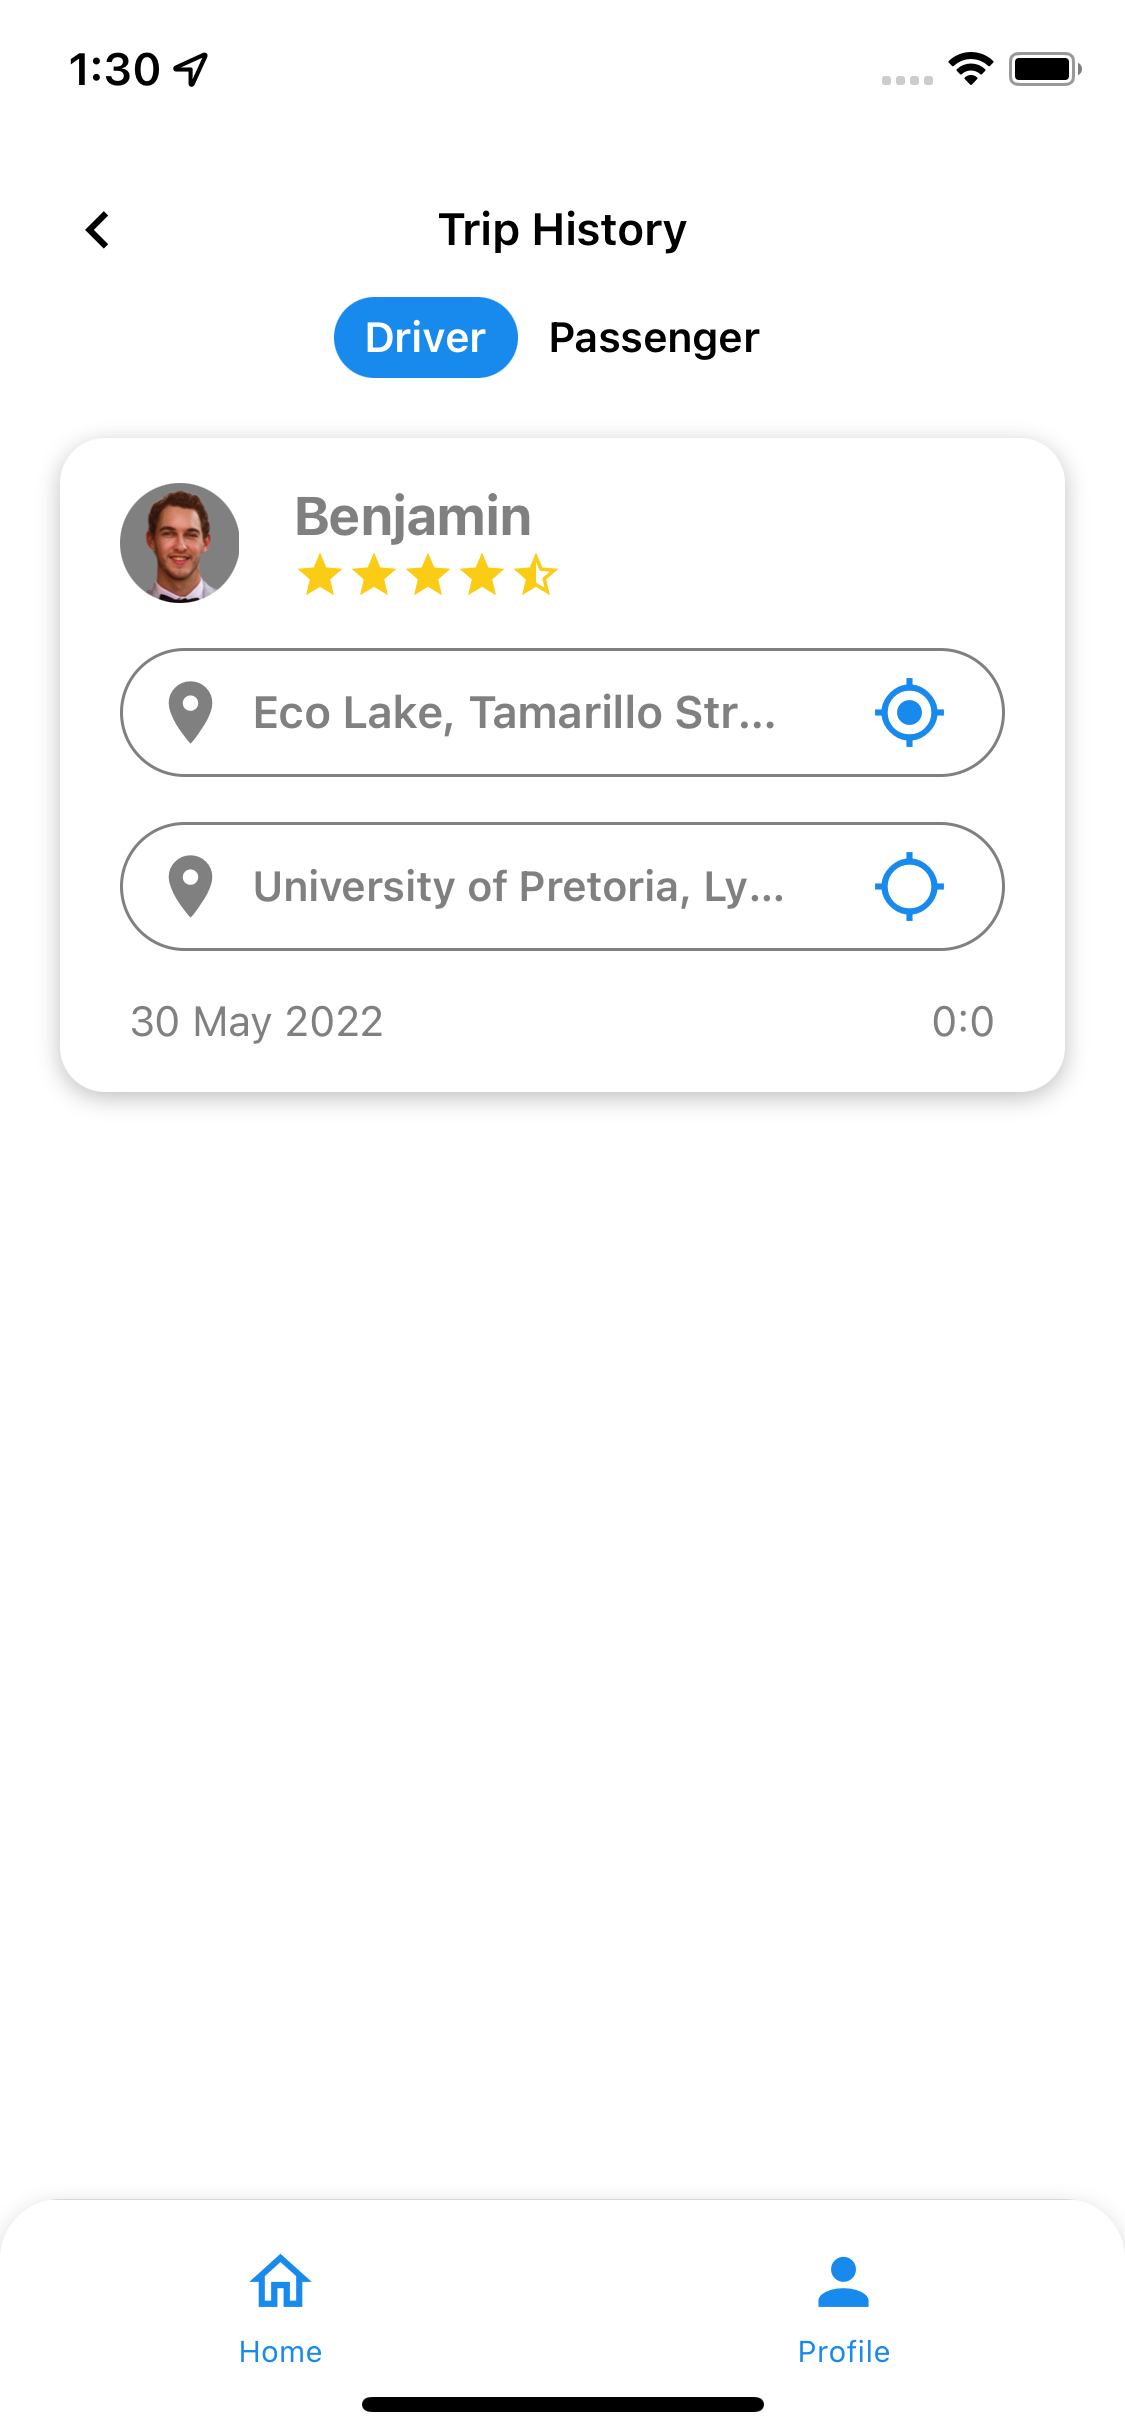
\includegraphics[height=10cm]{images/history_driver.png}
\end{center}
If the user wishes to know more information about the previous trip, they can just click on the trip card and they will be directed to the trip details page, which shows more information about the trip.
\vspace{1cm}

\subsection{Trip details}
The trip details page provides the user with all the necessary information about a trip:
\begin{itemize}
    \item Start and End location
    \item Price per seat
    \item Number of seats available
    \item Date and time of the trip
    \item Driver’s information: when clicked they will be taken to the driver’s profile page
    \item The user is also able to request to be apart of the trip by clicking on the Book Ride button which is located at the bottom of the screen.
    \item Shows the Start and end location on the map.
\end{itemize}
\begin{center}
  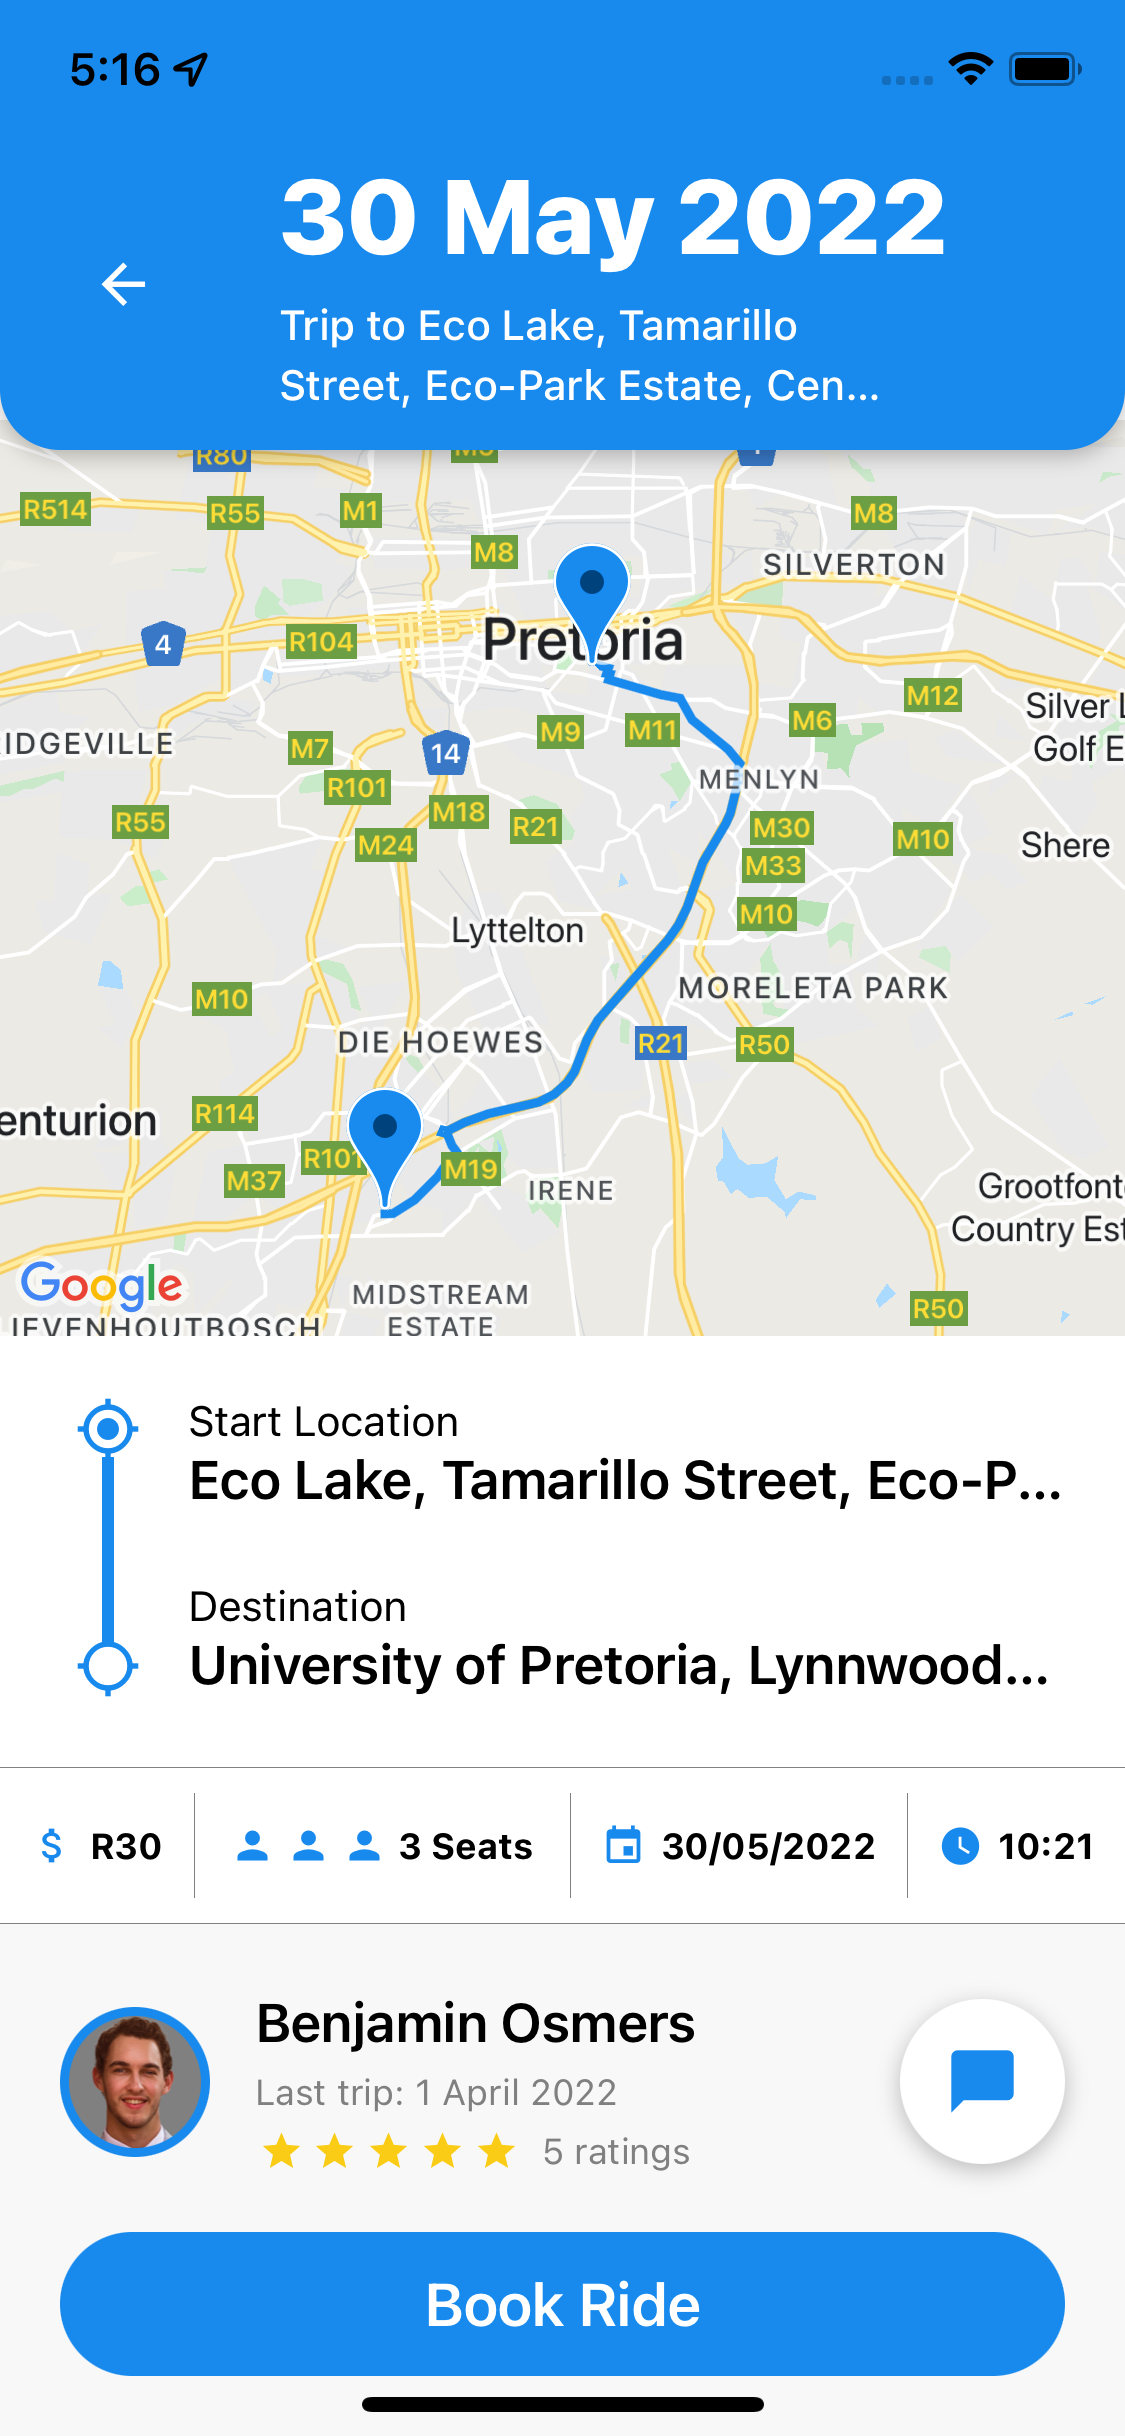
\includegraphics[height=10cm]{images/map_directions.png}
\end{center}

\subsection{Payment}
When clicking the shopping cart icon on the homepage, the user will be directed to a checkout screen whereby they are able to make payment for trips that they want to be apart of. The payment screen is divided into two tabs : Confirmed Trips and Requested Trips.

\subsubsection{Confirmed Trips}
In order for a trip to be classified as a confirmed trip, the driver of the trip has to accept the user’s (passenger) request to be a part of the trip. To view confirmed trips, the user must click on the confirm tab which is located at the top of the screen. A list of confirmed trips are displayed to the user, below the trip card is button titled “Pay Now”. When the user clicks on this button they will be directed to the credit card page.
\begin{center}
  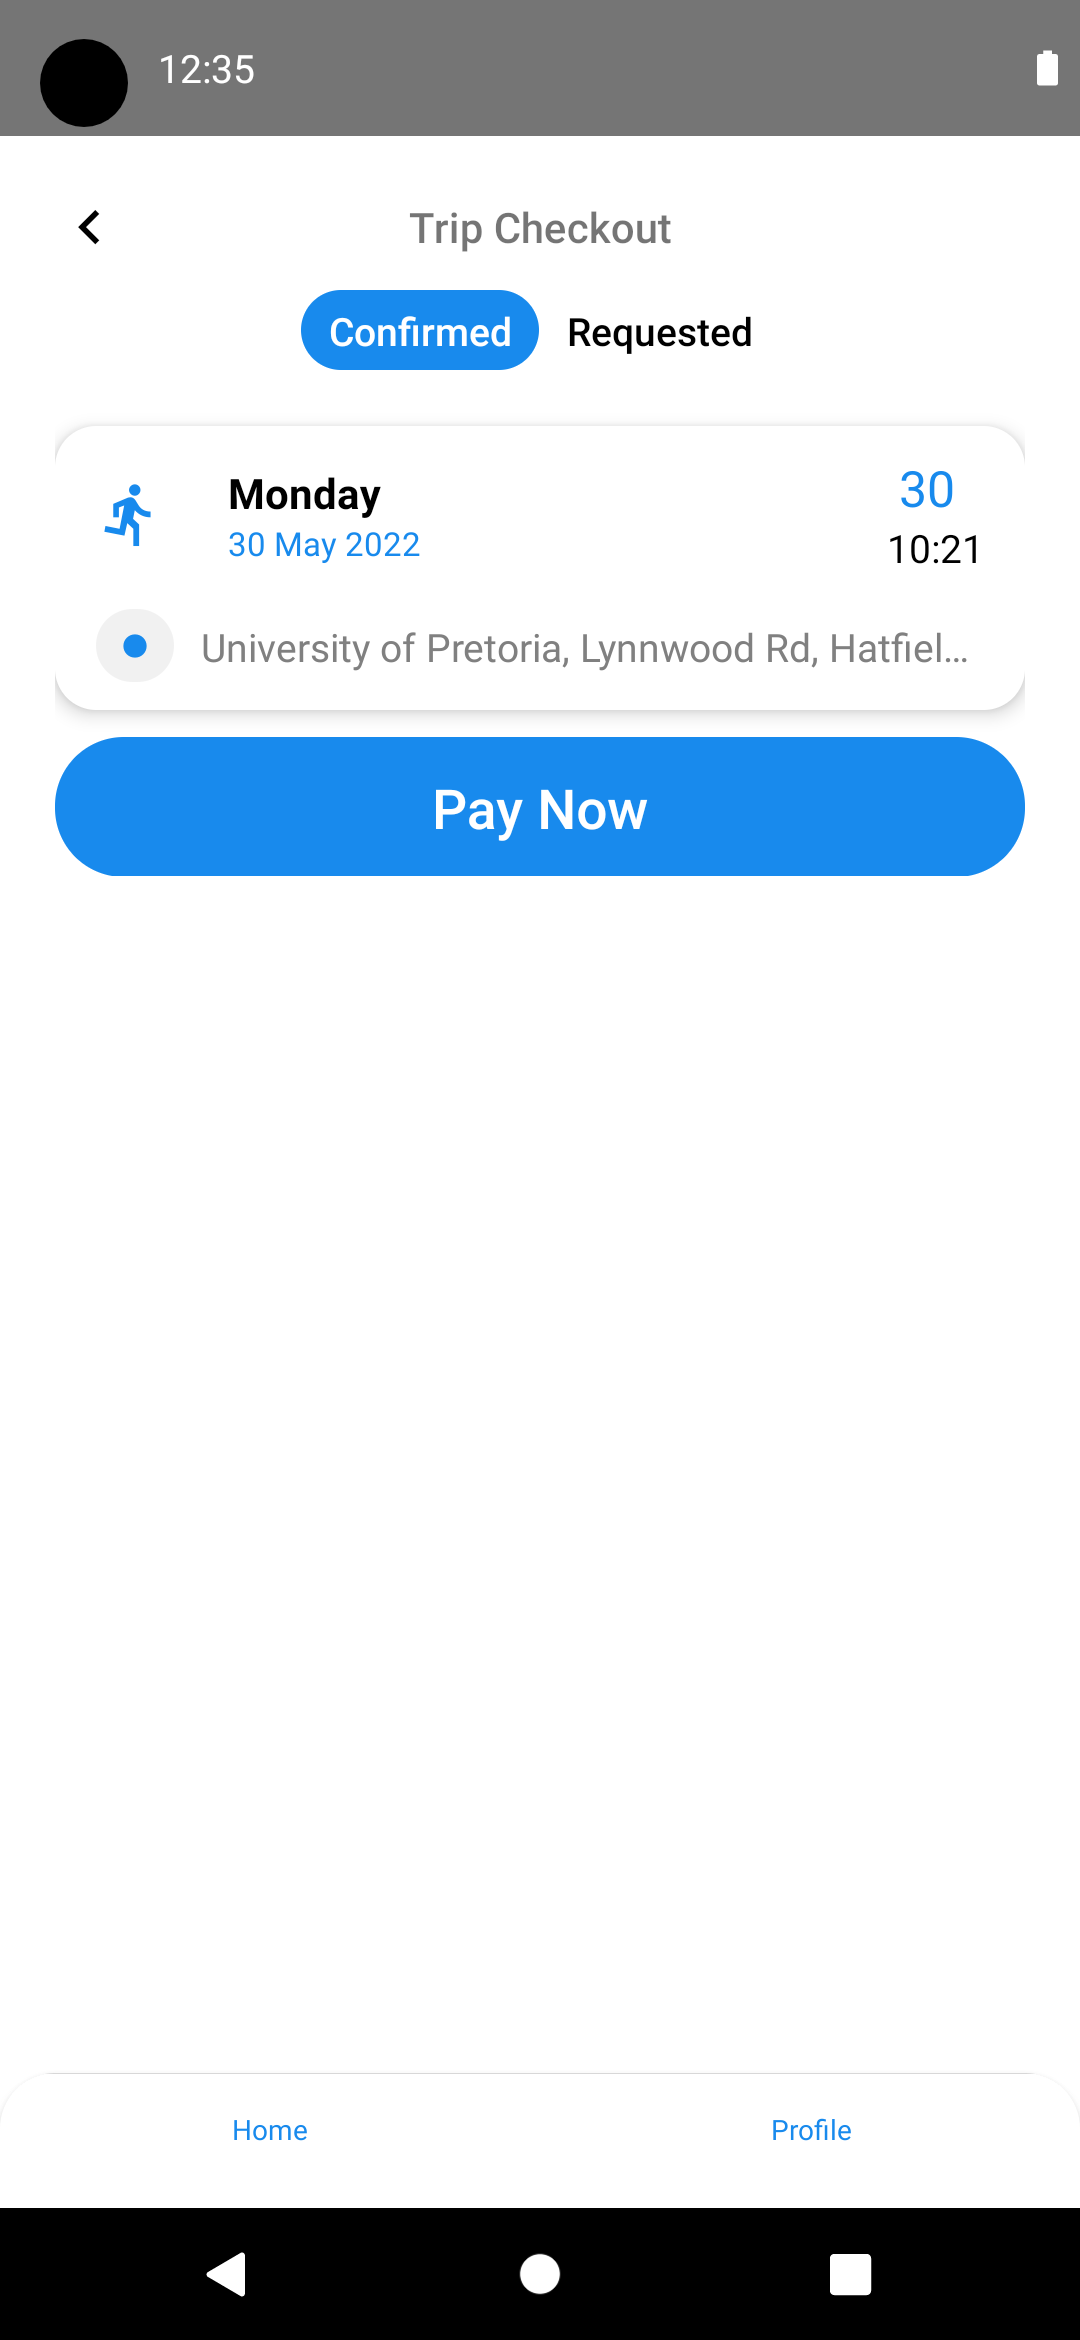
\includegraphics[height=10cm]{images/confirmed.png}
\end{center}
\vspace{1cm}

\subsubsection{Requested Trips}
For a trip to be classified as a requested trip, the driver of the trip has not yet accepted/ declined the user’s (passenger) request to be a part of the trip. To view requested trips, the user must click on the requested tab which is located at the top of the screen. A list of requested trips is displayed to the user. The user is not provided with the opportunity to pay for a requested trip, as the trip has not yet been confirmed. If a user pays for an unconfirmed trip, they could lose their money if the driver decides to decline their request.
\begin{center}
  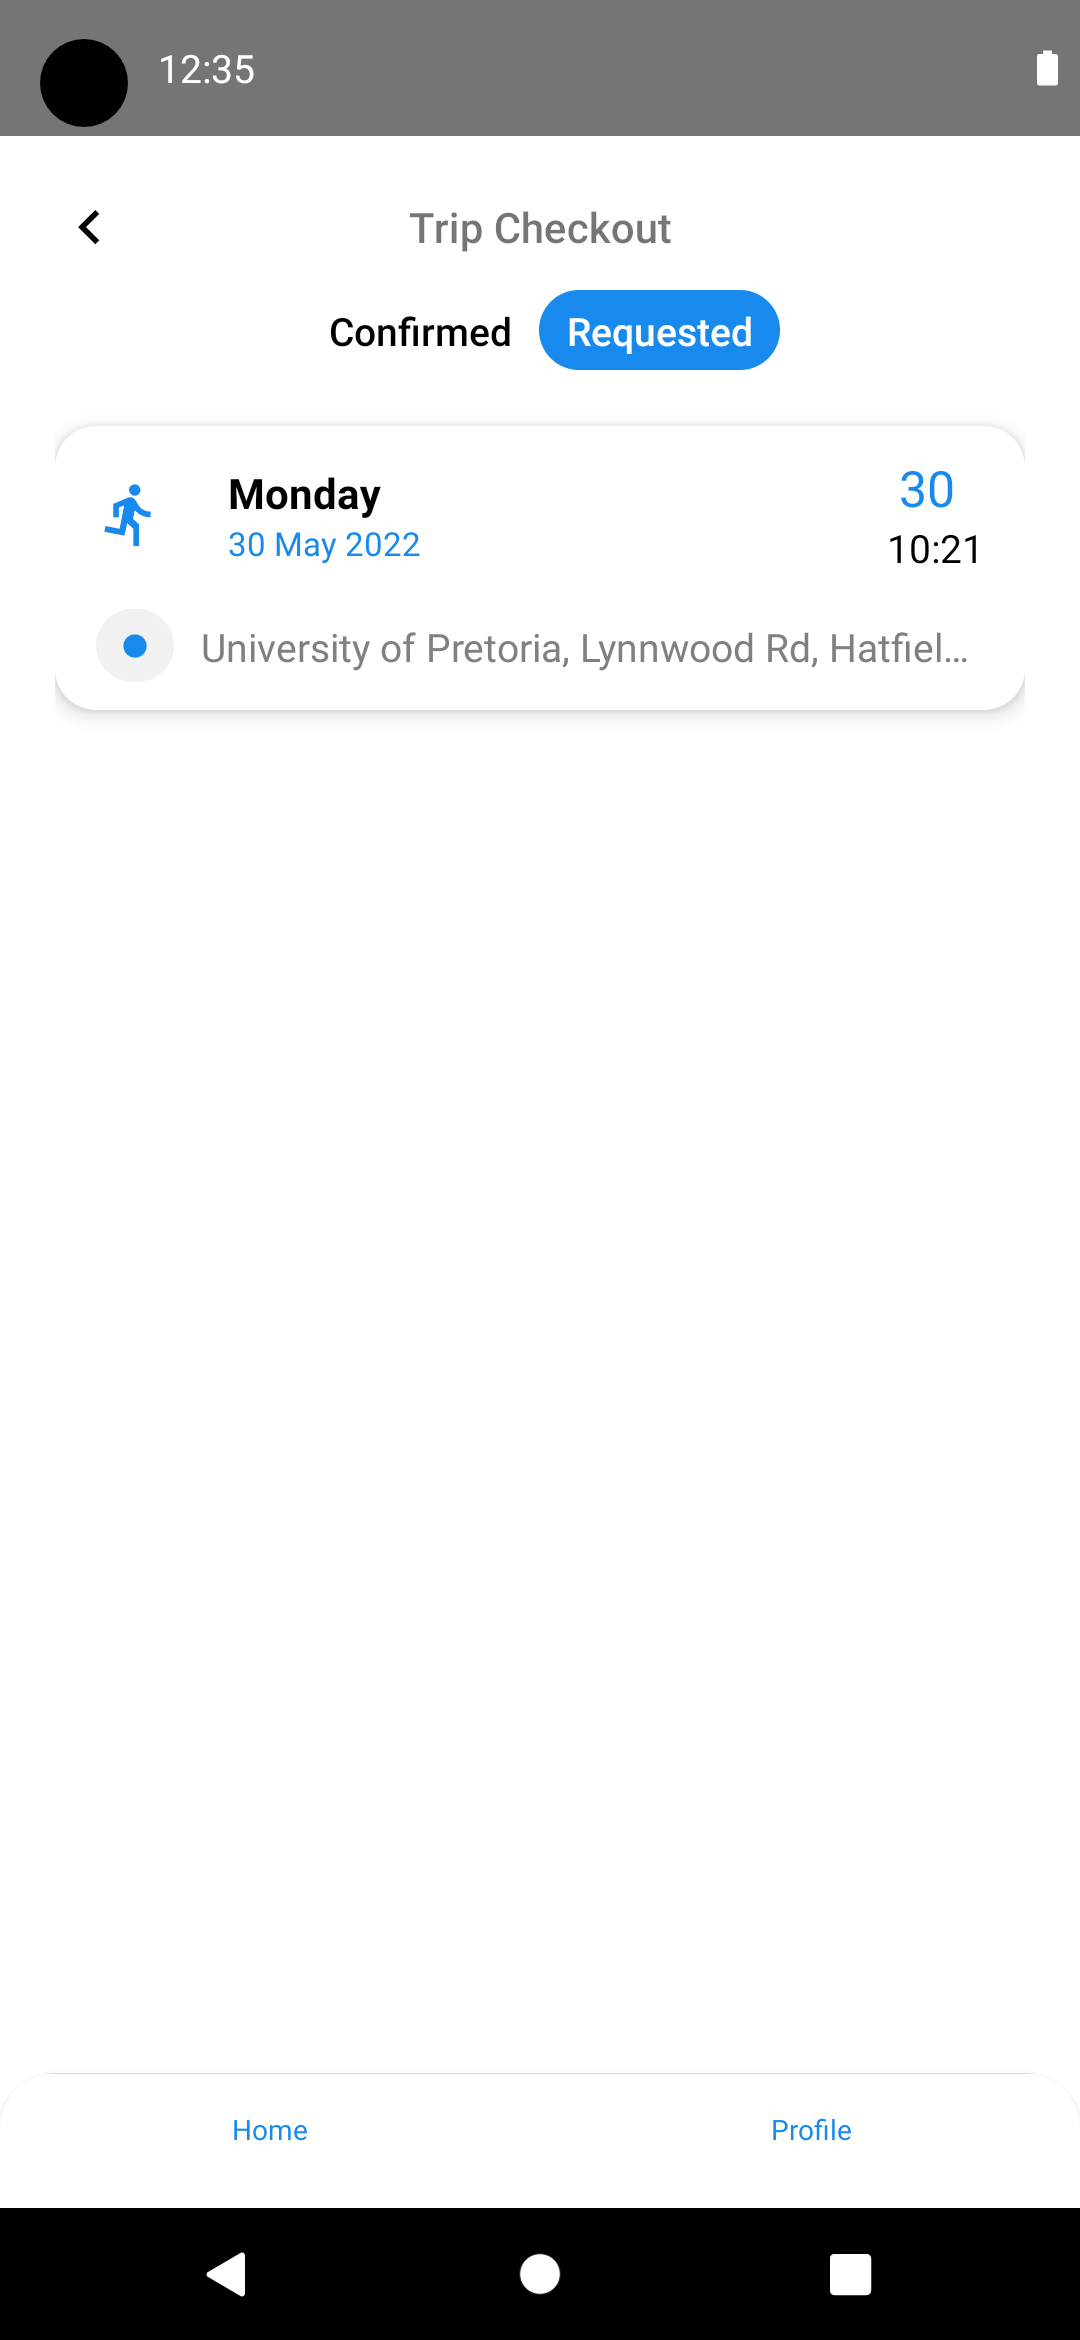
\includegraphics[height=10cm]{images/requested.png}
\end{center}
\vspace{1cm}
In order to view more information about the trip, the user can simply click on the trip card and they will be directed to the trip details page.


\subsubsection{Credit Card}
The user will be directed to this page when they click on the “Pay Now” button which is located on the check out page of confirmed trips. In order to make a payment, the user is required to enter their card number, card holder name, expiration date and CVC number (keyboard input). Once all the information is entered and validated, a confirm payment button will appear at the bottom of the screen. The user can click this button when they are ready to make payment for their trip.
\begin{center}
  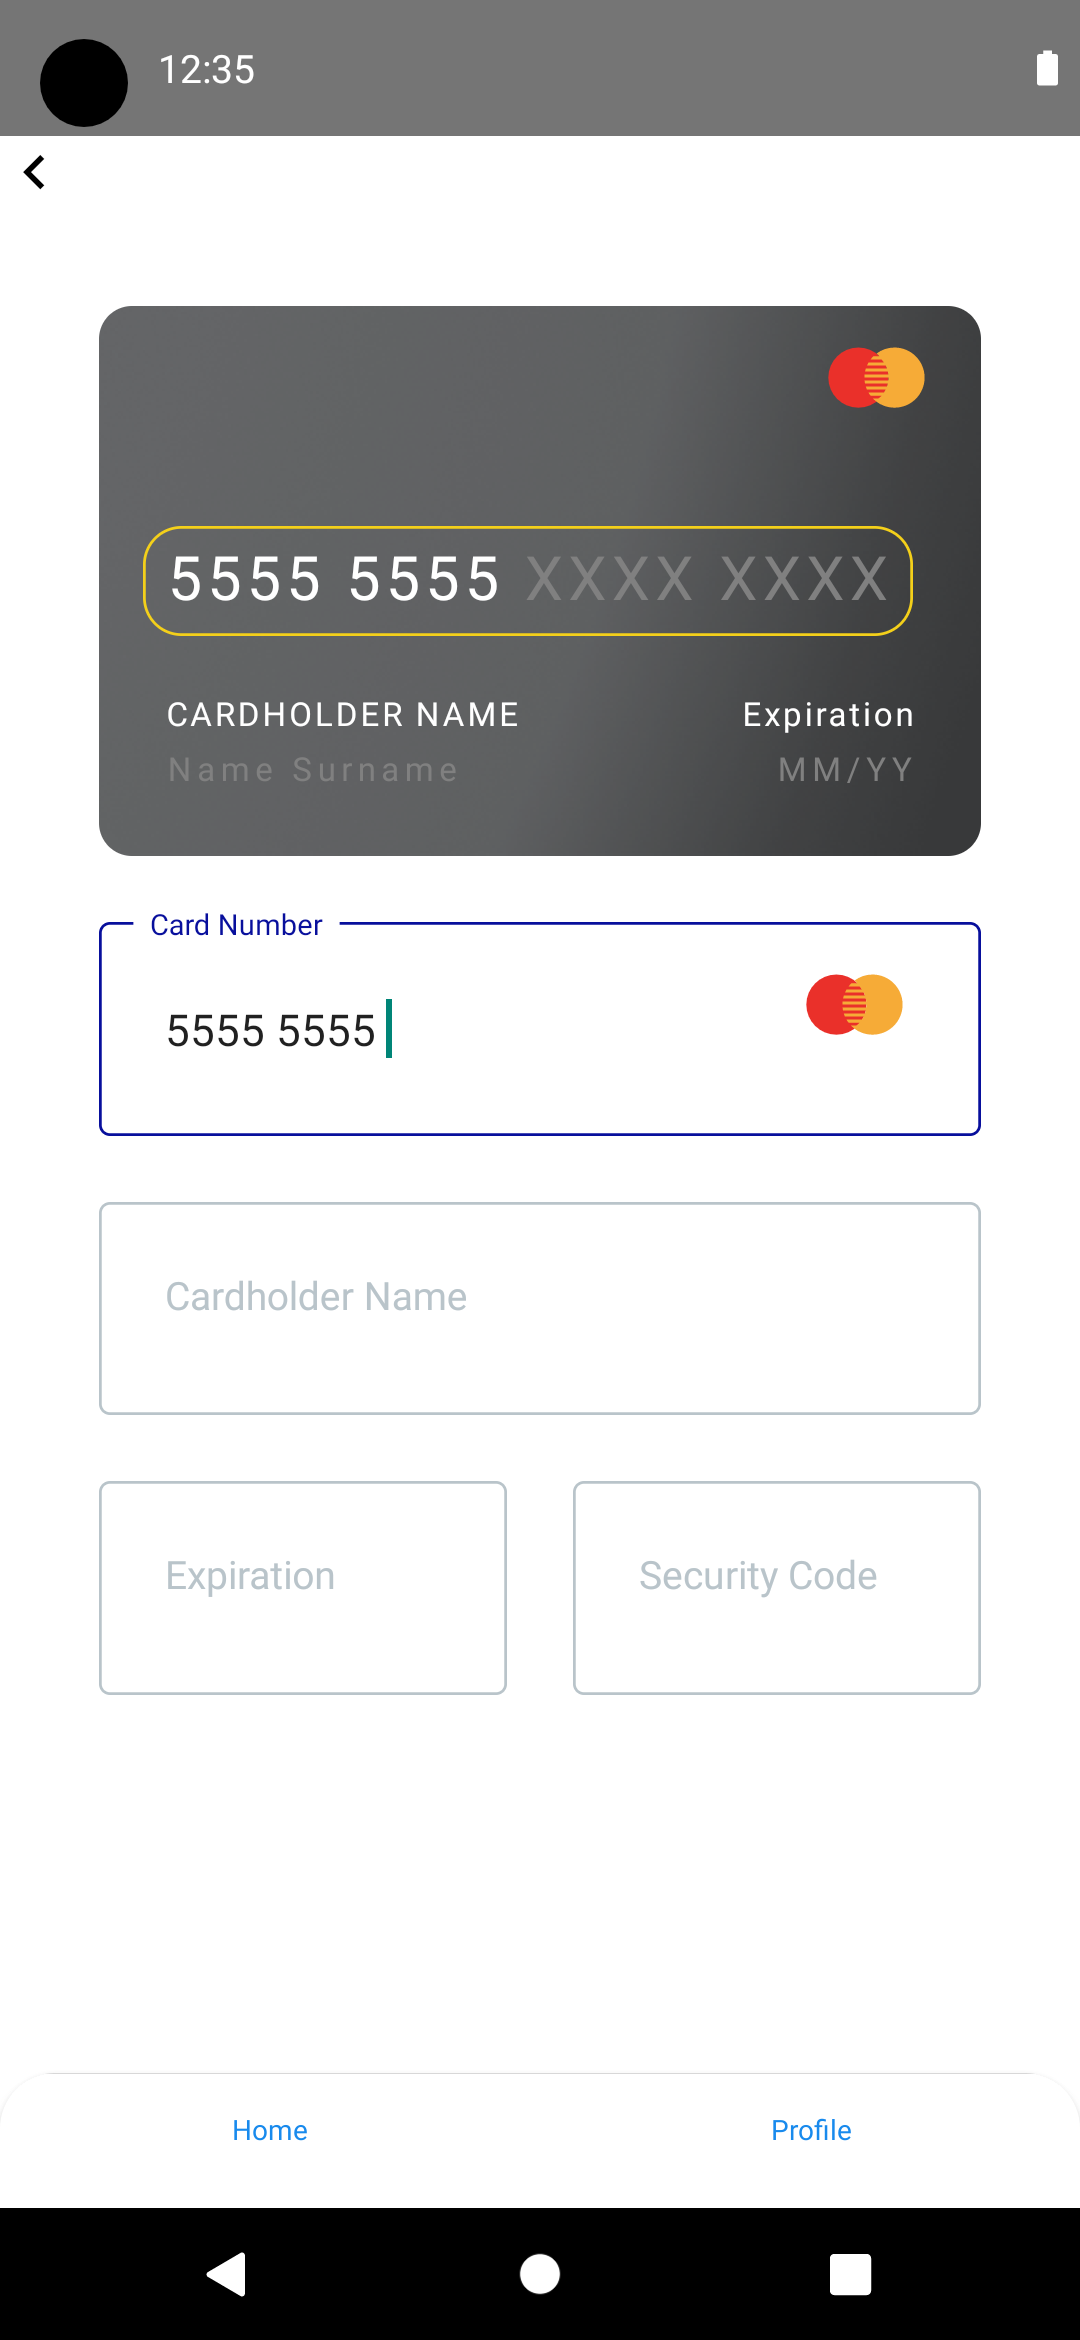
\includegraphics[height=10cm]{images/credit-card.png}
\end{center}
\vspace{1cm}
\end{document}